\documentclass{article}

% =========================
% Preamble (shared)
% =========================
\usepackage[
  paperwidth=210mm,
  paperheight=297mm,
  left=13.5mm,
  right=13.5mm,
  top=25mm,        % expanded top margin
  bottom=25mm      % expanded bottom margin
]{geometry}

% Line numbers
\usepackage{lineno}
\linenumbers

% Double spacing
\usepackage{setspace}
\doublespacing

% Page number top right
\usepackage{fancyhdr}
\pagestyle{fancy}
\fancyhf{}                          % clear all header/footer fields
\fancyhead[R]{\thepage}             % page number top right
\renewcommand{\headrulewidth}{0pt}  % remove header rule
\renewcommand{\footrulewidth}{0pt}  % remove footer rule
\fancypagestyle{plain}{%            % fix page 1
  \fancyhf{}%
  \fancyhead[R]{\thepage}%
  \renewcommand{\headrulewidth}{0pt}%
  \renewcommand{\footrulewidth}{0pt}%
}

\usepackage{soul,xcolor}
\sethlcolor{yellow}
% use this for adding comments since bold is a little unwieldy
% \hl{This sentence will be highlighted in whatever color we chose above.}
% Evie highlights
\newcommand{\eh}[1]{%
{\sethlcolor{cyan!30}\hl{#1}}%
}
% Scott highlights
\newcommand{\pink}[1]{%
{\sethlcolor{pink!50}\hl{#1}}%
}
\usepackage[T1]{fontenc}
\usepackage{graphicx}
%\usepackage[numbers,super,sort&compress]{natbib}
%\setcitestyle{citesep={,}}
\usepackage[numbers,square]{natbib}

\usepackage[section]{placeins}
\usepackage{afterpage}
\usepackage{caption}
\captionsetup{
  justification=justified,
  singlelinecheck=false,
  labelfont=bf,
  labelsep=period,
  font=footnotesize
}
% Custom figure reference helpers
\newcommand{\Figref}[1]{Figure~\ref{#1}}
\newcommand{\figref}[1]{Fig.~\ref{#1}}
\usepackage{hyperref}

\begin{document}

% =========================
% Main manuscript
% =========================

\title{Paper Draft}
\author{Henry et al}
\date{} % keep if you want to suppress date

\maketitle

\section{Introduction}

% This was ripped straight from Shaposhnikov, but don't think I need it anyway:
% Aging is a complex biological process characterized by the progressive decline of physiological functions and increased susceptibility to disease, ultimately leading to death {Shaposhnikov, 2022 159}.
Over the past several decades, research across diverse model organisms, from yeast and nematodes to flies and mammals, has revealed that the rate of aging is not fixed but can be modulated by genetic, environmental, and pharmacological interventions \citep{gems2013}. 
Remarkably, many of the molecular pathways that regulate lifespan are highly conserved, suggesting that fundamental mechanisms of aging may be shared across taxa \citep{lopez-otin2013}.

While much of aging research has involved direct perturbation of these conserved pathways, an intriguing dimension of aging biology was revealed by the discovery that sensory perception can modulate lifespan independent of the physical acts associated with perceived stimuli \citep{pontillo2025, gendron2020, miller2020}. 
Studies in the nematode worm, \textit{Caenorhabditis elegans}, and the vinegar fly, \textit{Drosophila melanogaster}, have demonstrated that sensory cues related to food, mates, and even the presence of dead conspecifics can initiate physiological changes that influence patterns of aging \citep{gendron2014, chakraborty2019, libert2007,hernandez-lima2025, miller2022}. 
These effects are mediated by neuronal circuits that emanate from sensory tissues and interface with deeper regions of the central nervous system, ultimately engaging conserved neuromodulators, including biogenic amines and neuropeptides, that influence metabolism, stress resistance, and longevity \citep{chakraborty2019, miller2020, miller2022}. 

In at least some cases, sensory perception has been shown to modulate lifespan through the motivational states \textit{per se} that it influences. 
For example, the neuropeptide F system, homologous to mammalian neuropeptide Y, is a component of reward- and stress-related processing, and its activation can reduce starvation resistance and shorten lifespan \citep{ryvkin2024, gendron2014}.
Sensory perception of potential mates shortens lifespan in male flies through circuits involving NPF signaling, whereas successful mating reverses these effects \citep{gendron2014}, suggesting that an unresolved expectation of reward can influence lifespan. 
Insatiable hunger also slows aging, despite promoting behaviors normally associated with decreased lifespan\citep{weaver2023a}. 
These observations indicate that identifying the neural circuits that interpret and integrate sensory inputs, as well as how they generate conserved internal states that prescribe physiological outcomes, may provide new insight into healthy aging.

In \textit{Drosophila}, one neural substrate has recently emerged as a strong candidate for such an interpretive center: the ellipsoid body (EB). 
The EB resides within the central complex, a region that shares functional and organizational homology with the mammalian basal ganglia \citep{strausfeld2013}. 
The EB is subdivided into concentric domains innervated by six major classes of ring neurons (termed "ER" or "R" neurons) that process visual, thermal, mechanosensory, and circadian information \citep{hulse2021, buhl2021, yan2023}.
Exposure of flies to dead conspecifics, termed “death perception,” reduces fat stores, lowers starvation resistance, and shortens lifespan in a manner that requires visual function and serotonin signaling through 5-HT2A-expressing R2 and R4 neurons \citep{chakraborty2019}.
Insulin-like peptides, as well as the insulin-responsive transcription factor dFOXO, are required for aging effects of death perception, suggesting that EB ring neurons interface with conserved metabolic pathways implicated in lifespan control \citep{gendron2023}. 
Additional roles for EB ring neuron classes in locomotor control, sleep, visual memory, and state-dependent action selection, suggest that it is well-positioned to link myriad sensory representations to organismal state \citep{ofstad2011, yan2023, buhl2021, kottler2019}.

The extent to which the results in \textit{Drosophila} may illuminate similar processes in other taxa may hinge on the nature of the EB's role in influencing health-related outcomes. 
One possibility is that these neurons function primarily as passive conduits or gates for lifespan-altering sensory information: if their function is disrupted, flies may simply fail to perceive \citep{seelig2013, omoto2017} or internally represent salient stimuli, and phenotypes normally induced by those stimuli would not manifest. 
A more intriguing alternative is that the EB is an instructive modulator of aging-related processes, and direct manipulation of ring neuron activity, independent of external sensory input, would be sufficient to alter aging. 
It is this latter case that, if true, suggests translational potential for targeting central neuromodulatory and sensory-integration mechanisms in aging research.
% EH: You asked for a ref in this last sentence, but i'm not sure what you have in mind. An example where they targeted sensory integration mechanisms based on invert research, or?

Here, we use a variety of optogenetic tools, which enable temporally precise activation or inhibition of genetically-defined neuronal populations, to show that \textit{Drosophila} EB ring neuron populations are prescriptive modulators of aging that encode behaviorally meaningful information and orchestrate diverse transcriptional and metabolic responses throughout the animal. 
Our findings indicate that these neurons can act as active regulators of pro-longevity physiology rather than only as conduits for perception-dependent aging signals. 
Activation of R2 neurons, inhibition of R4d neurons, and simultaneous activation of R2 and R4 neurons each extends lifespan in males and females, but these manipulations produce divergent transcriptional responses in head tissues, including distinct effects on insulin signaling, stress-response, and metabolic pathways. 
Despite these molecular differences, we detect no consistent changes in feeding, fat storage, locomotor activity, or climbing ability that account for the longevity effects, arguing against a simple explanation based on overt energetic or behavioral shifts. 
Valence assays further show that R2 activation alone produces a negatively-valenced state, whereas combined R2/R4 activation produces a positively-valenced state, indicating that distinct neural states with different immediate behavioral consequences can converge on increased lifespan. 
Transcriptomic and metabolomic profiling of peripheral tissues further reveals that R2 activation drives systemic metabolic remodeling, including suppression of proliferative programs and upregulation of electrochemical and membrane homeostasis pathways not observed in head tissues, demonstrating that EB ring neuron activity induces tissue-specific responses throughout the fly.
Together, these findings support a model in which the ellipsoid body serves as an integrative neural locus through which sensory and state-related processes can influence aging via multiple downstream physiological programs.



\title{Paper Draft}
\author{Henry et al}
\date{} % keep if you want to suppress date

\maketitle

\section{Introduction}

% This was ripped straight from Shaposhnikov, but don't think I need it anyway:
% Aging is a complex biological process characterized by the progressive decline of physiological functions and increased susceptibility to disease, ultimately leading to death {Shaposhnikov, 2022 159}.
Over the past several decades, research across diverse model organisms, from yeast and nematodes to flies and mammals, has revealed that the rate of aging is not fixed but can be modulated by genetic, environmental, and pharmacological interventions \citep{gems2013}. 
Remarkably, many of the molecular pathways that regulate lifespan are highly conserved, suggesting that fundamental mechanisms of aging may be shared across taxa \citep{lopez-otin2013}.
While much of aging research has involved direct perturbation of these conserved pathways, an intriguing dimension of aging biology was revealed by the discovery that sensory perception can modulate lifespan independent of the physical acts associated with perceived stimuli \citep{pontillo2025, gendron2020, miller2020, garratt2022}. 
Studies in the nematode worm, \textit{Caenorhabditis elegans}, and the vinegar fly, \textit{Drosophila melanogaster}, have demonstrated that sensory cues related to food, mates, and even the presence of dead conspecifics can initiate physiological changes that influence patterns of aging \citep{gendron2014, chakraborty2019, libert2007, hernandez-lima2025, miller2022}. 
These effects are mediated by neuronal circuits that emanate from sensory tissues and interface with deeper regions of the central nervous system, ultimately engaging conserved neuromodulators, including biogenic amines and neuropeptides, that influence metabolism, stress resistance, and longevity \citep{chakraborty2019, miller2020, miller2022}. 

In at least some cases, sensory perception has been shown to modulate lifespan through the motivational states \textit{per se} that it influences. 
For example, the neuropeptide F system, homologous to mammalian neuropeptide Y, is a component of reward- and stress-related processing, and its activation can reduce starvation resistance and shorten lifespan \citep{ryvkin2024, gendron2014}.
Sensory perception of potential mates shortens lifespan in male flies through circuits involving NPF signaling, whereas successful mating reverses these effects \citep{gendron2014}, suggesting that an unresolved expectation of reward can influence lifespan. 
Insatiable hunger also slows aging, despite promoting behaviors normally associated with decreased lifespan \citep{weaver2023a}. 
These observations indicate that identifying the neural circuits that interpret and integrate sensory inputs, as well as how they generate conserved internal states that prescribe physiological outcomes, may provide new insight into healthy aging.

In \textit{Drosophila}, one neural substrate has recently emerged as a strong candidate for such an interpretive center: the ellipsoid body (EB). 
The EB resides within the central complex, a region that shares functional and organizational homology with the mammalian basal ganglia \citep{strausfeld2013}. 
The EB is subdivided into concentric domains innervated by six major classes of ring neurons (termed "ER" neurons) that process visual, thermal, mechanosensory, and circadian information to drive behavioral outputs \citep{hulse2021, buhl2021, yan2023}. 
Additional roles for EB ring neuron classes involve locomotor control, sleep, visual memory, and state-dependent action selection, suggest that it is well-positioned to link myriad sensory representations to organismal state \citep{ofstad2011, yan2023, buhl2021, kottler2019}.
Recent work has implicated this structure in aging biology.
Exposure of flies to dead conspecifics, termed “death perception,” reduces fat stores, lowers starvation resistance, and shortens lifespan in a manner that requires visual function and serotonin signaling through 5-HT2A-expressing ER2 and ER4 neurons \citep{chakraborty2019}.
Insulin-like peptides, as well as the insulin-responsive transcription factor dFOXO, are required for aging effects of death perception, suggesting that EB ring neurons interface with conserved metabolic pathways implicated in lifespan control \citep{gendron2023}. 


The extent to which the results in \textit{Drosophila} may illuminate similar processes in other taxa may hinge on the nature of the EB's role in influencing health-related outcomes. 
One possibility is that these neurons function primarily as passive conduits or gates for lifespan-altering sensory information: if their function is disrupted, flies may simply fail to perceive \citep{seelig2013, omoto2017} or internally represent salient stimuli, and phenotypes normally induced by those stimuli would not manifest. 
A more intriguing alternative is that the EB is an instructive modulator of aging-related processes, and direct manipulation of ring neuron activity, independent of particular sensory input, would be sufficient to alter aging. 
If true, this latter case would implicate the EB and functionally similar structures---i.e., central hubs of neuromodulation and sensory integration---as rich targets for aging research.

Here, we use a variety of optogenetic tools, which enable temporally precise activation or inhibition of genetically-defined neuronal populations, to show that \textit{Drosophila} EB ring neuron populations are prescriptive modulators of aging that encode behaviorally meaningful information and orchestrate diverse transcriptional and metabolic responses throughout the animal. 
Our findings indicate that these neurons can act as active regulators of pro-longevity physiology rather than only as conduits for perception-dependent aging signals. 
Activation of ER2 neurons, inhibition of ER4d neurons, and simultaneous activation of ER2 and ER4 neurons each extends lifespan in males and females, but the manipulations produce divergent transcriptional responses in head tissues, including distinct effects on insulin signaling, stress-response, and metabolic pathways. 
Despite these molecular differences, we detect no consistent changes in feeding, fat storage, locomotor activity, or climbing ability that account for the longevity effects, arguing against a simple explanation based on overt energetic or behavioral shifts. 
Valence assays further show that ER2 activation alone produces a negatively-valenced state, whereas combined ER2/ER4 activation produces a positively-valenced state, indicating that distinct neural states with different immediate behavioral consequences can converge on increased lifespan. 
Transcriptomic and metabolomic profiling of peripheral tissues further reveals that ER2 activation drives systemic metabolic remodeling, including suppression of proliferative programs and upregulation of electrochemical and membrane homeostasis pathways not observed in head tissues, demonstrating that EB ring neuron activity induces tissue-specific responses throughout the fly.
Together, these findings support a model in which the ellipsoid body serves as an integrative neural locus through which sensory and state-related processes can influence aging via multiple downstream physiological programs.

\section{Results}

\subsection*{Manipulating ER2 and ER4 neurons in the ellipsoid body extends fly lifespan}

To determine if the activity of ellipsoid body ring neurons is capable of modulating lifespan, we performed a series of experiments in which the activity of EB neurons was manipulated, with the following considerations informing our experimental design. 

First, we sought to eliminate potential developmental effects and to restrict neuronal manipulations to adults with a developed central complex \citep{lovick2017}. 
Second, we wanted to avoid tools that require introducing confounding factors, such as high temperatures, which can significantly affect lifespan and obscure treatment effects on aging \citep{miquel1976}. 
Third, we wanted the flexibility to perform acute, cyclic, or chronic manipulations in ethologically-relevant contexts involving lifespan, behavior, and health assays. 
To accommodate these requirements, we adopted an optogenetic \citep{govorunova2015} approach to apply different treatment paradigms to freely-moving and fully developed adults by changing light-activation parameters and exposure times. 
To assay lifespans, we housed flies in custom optogenetic rigs with programmable, interchangeable LED bars, accommodating different channelrhodopsins and allowing us to either activate \citep{klapoetke2014} or inhibit \citep{mohammad2017} targeted neuron populations. 
Unless otherwise noted, flies in all treatment paradigms were exposed to light activation (40 Hz, 32\% duty cycle) during ZT 0-12 of a 12:12 light:dark cycle, beginning at 3 days post-eclosion and continuing throughout adulthood, promoting a normal circadian rhythm and restricting neuronal manipulations to periods when flies would typically be alert and interacting with their environment (\figref{fig:lifespanfig}A).
Flies were otherwise maintained using standard husbandry conditions \citep{linford2013}. 

We focused our investigation on ER2 and ER4, specifically ER4d, neurons, as these are required for the perception of dead conspecifics to modulate lifespan \citep{gendron2023} and for food perception to enhance starvation resistance \citep{luo2021}. 
When flies expressing UAS-CsChrimson \citep{klapoetke2014} in ER2 neurons (ER2>Chr) were exposed to red light during subjective day, we observed a significantly extended lifespan in both females and males compared to siblings aged in the dark (\figref{fig:lifespanfig}B). 
This effect was not observed in genotype control flies that did not express CsChrimson, ruling out general lifespan-extending effects of red light and indicating a direct effect of neuronal activation. 
Activation of ER4d neurons had little meaningful effect on lifespan (\figref{fig:lifespansupp}A). 
However, when ER4d neurons were inhibited by exposing flies expressing the anion channelrhodopsin GtACR1 \citep{mohammad2017} to green light during subjective day, lifespan was significantly extended in both females and males (\figref{fig:lifespanfig}C). 
These results should be interpreted with caution, however, because we observed that exposure to high-intensity green light caused a significant reduction in lifespan in all cohorts (roughly 50\% in females and 33\% in males). 
Nevertheless, GtACR1 flies lived modestly but significantly longer than control flies in the light, a pattern that was not observed in the dark.

% Got rid of the "ixn p-value" notes here since we decided not to use Cox regressions
The observation that ER2 and ER4d neuron activation had different effects on lifespan was somewhat unexpected given that measures of ER2 and ER4 neuronal activity were both observed to be higher following exposure to dead conspecifics \citep{gendron2023}, which accelerates aging \citep{chakraborty2019}. 
We therefore decided to examine the effect of simultaneous activation of ER2 and ER4 (comprising ER4d and ER4m subpopulations) using a split-GAL4 driver. 
To our surprise, simultaneously activating both populations extended lifespan in males and females (\figref{fig:lifespanfig}D) to a greater extent than did ER2 activation alone. 
In this experiment, red light exposure modestly increased lifespan of CsChrimson-expressing flies as well as their genotypic controls, but the increase in lifespan was significantly greater in CsChrimson flies. 
% Highlights - need Cox regression or something?
Given the substantial increase in lifespan observed following simultaneous ER2/ER4 activation, we asked whether even broader manipulation of ellipsoid body neurons would recapitulate or even potentiate the lifespan extension that we observed following ER2 and ER2/ER4 neuron activation. 
Using a driver that targets additional EB neuron populations, including at least R3 neurons, we observed that broader EB inhibition had no effect on lifespan (\figref{fig:lifespanfig}E, left) and activation increased lifespan to an equal or lesser extent than ER2 or ER2/ER4 activation alone (\figref{fig:lifespanfig}E, right). 

Together, these data demonstrate that enhanced EB neural activity promotes longevity primarily through ER2 and ER4 neurons, supporting the notion that the ellipsoid body is an instructive generator of lifespan-modulating signals. 
These results may be interpreted in the context of known activity patterns of ER2/ER4 in other contexts. 
Ishimoto et al. reported that ER2, ER4m, and ER4d neurons work together in an incoherent type 1 feedforward loop (I1-FFL) \citep{ishimoto2020}. 
Upon simultaneous activation of ER2/ER4m and ER4d, ER4d signaling initially increased, but sustained activity of GABAergic ER2 and ER4m neurons gradually suppressed ER4d activity. 
If optogenetic activation recruits ER2/ER4 in this feedforward fashion, it may be that ER2 activation, ER2/ER4 activation, and ER4d inhibition are effectively the same intervention. 
Alternatively, they may engage partially or fully distinct pathways that converge on extended lifespan via different downstream mechanisms. 

\subsection*{Different ring neuron manipulations produce distinct transcriptional profiles}

To investigate how ER2 and ER4 neurons modulate aging and whether they do so via similar or distinct mechanisms, we performed bulk RNA-sequencing on brain-enriched tissues of female flies after one week of ER2 activation, ER4d inhibition, or ER2/ER4 activation, under the same conditions used in the lifespan assays described above. 
We chose to sample flies after one week of optogenetic manipulation to avoid survivorship bias that might arise at later time points while still allowing time for physiological differences to manifest. 
Flies were transferred directly from experimental rigs to liquid nitrogen, then decapitated by vortexing, and heads were collected with a sieve. 
Five biological replicates of 10 heads were collected for CsChrimson/GtACR1 and control genotypes from flies maintained either in constant darkness or channel-activating red/green lights during the 12 hours of subjective day. 
Whole head samples comprised primarily brain tissue, although other tissues were present, including the head fat body. 

We used the DESeq2 package in R \citep{love2014} to identify transcriptional changes associated with enhanced ER2 neural activity.
We specified a statistical model in which genotype (CsChrimson, control) and light stimulation (yes, no) served as main effects. 
A Light $\times$ Genotype interaction term was used to identify significant transcriptional changes that were specific to light-driven channelrhodopsin stimulation, and these were the primary focus of our analysis. 
After one week of ER2 neuron activation, we identified 123 genes (70 downregulated and 53 upregulated) whose expression values exhibited experiment-wise interaction p-values less than our cutoff of p < 0.01. 
Expression data from these genes produced clear separation of samples by treatment, indicating strong reproducibility across each of the five replicates (\figref{fig:seqfig}A). 
Hierarchical clustering revealed that samples from flies with activated ER2 neurons (i.e. ER2>CsChrimson flies exposed to red light) formed a distinct group from flies without neuronal activation, including CsChrimson-expressing flies maintained in constant darkness as well as control genotype samples maintained in either darkness or red light. 

Despite a stringent threshold (requiring a false discovery rate < 0.01), we observed that one week of ER2 neuron activation drove broad but pathway-enriched changes in the head. 
GO analysis of upregulated genes revealed enrichment for ribosome biogenesis and rRNA processing, insulin signaling, and response to starvation (\figref{fig:seqfig}B). 
Downregulated genes were enriched for protein folding and ER stress response pathways (\figref{fig:seqfig}C). 
Together, these results suggest that activation of ER2 neurons induces a distinct metabolic state in the head, characterized by altered nutrient signaling and reduced ER stress. 
It also caught our attention that many of the differentially-expressed genes have been implicated in aging biology, with several known to modulate aging directly. 
For example, we observed the upregulation of multiple genes consistent with dampened insulin-like signaling (e.g., \textit{foxo}, \textit{Thor} (encoding d4E-BP), \textit{InR}, \textit{dilp6}) \citep{partridge2010}; upregulation of autophagy-related genes such as \textit{Atg101} \citep{guo2019}; upregulation of \textit{ImpL2}, an IIS antagonist which has been linked to lifespan extension \citep{alic2011}; and higher levels of \textit{Cbs}, which encodes the rate-limiting enzyme in the transsulfuration pathway and increases lifespan \citep{kabil2011}. 
Together, these results demonstrate that short-term, part-time activation (12L/12D) of a few dozen ER2 neurons drives significant changes in multiple aging-, nutrient-, and stress-response pathways. 

Following one week of ER4d silencing, far fewer genes were found to be differentially expressed (\figref{fig:seqfig}D), although ER4d-specific changes were likely masked by remarkably potent independent effects of intense green light exposure. 

As observed for the ER2 data, sample-based clustering grouped biological replicates as more closely related to each other than to samples from all other treatments, demonstrating reproducibility. 
Consistent with its significant negative effect on lifespan (\figref{fig:lifespanfig}C), green light exposure affected the expression of 1,817 genes regardless of genotype (experiment-wise p < 0.01). 
However, only 11 genes (9 downregulated and 2 upregulated) were associated with a significant p-value for the interaction term of the model, which indicates a differential response in flies with ER4d neurons silenced. 
Interestingly, in both genotypes, green light drove strong upregulation of multiple genes that encode heat shock proteins (e.g., \textit{Hsp23}, \textit{Hsp26}, \textit{Hsp27}, \textit{Hsp70Bb}), which was significantly muted in flies with ER4d neurons silenced. 
Other differentially-expressed genes following ER4d inhibition include the enzyme tyrosine hydroxylase (\textit{ple}), which catalyzes the rate-determining step in dopamine synthesis \citep{neckameyer1993}; the serine protease homolog \textit{scarface} \citep{prasad2018}; and several genes of unknown function. 
% Sugar promotes feeding via Scarface, note to self (2018)

% moved to Discussion: "Temeratures in our ventilated..." 
We next asked how transcriptional changes following simultaneous activation of ER2 and ER4 compared to manipulations of the individual neuron populations. 
When ER2 and ER4 neurons were activated simultaneously, we once again observed high reproducibility with replicate samples within treatments being clustered together and flies with activated ER2/ER4 neurons forming a cluster distinct from both genotype and light controls (\figref{fig:seqfig2}A). 
Using a false discovery rate-corrected cutoff of p < 0.01, we observed that ER2/ER4 activation resulted in roughly twice as many transcriptional changes as did ER2 activation alone (198 upregulated and 82 downregulated). 
A GO analysis of the upregulated genes was dominated by metabolic pathways related to amino acid metabolism as well as pentose-phosphate- and NADPH-generating processes (\figref{fig:seqfig2}B). 
We also observed an upregulation of several known lifespan-modulating genes involved in one carbon metabolism, including \textit{Cbs}, \textit{Gnmt}, \textit{Glyp}, \textit{Glys}, \textit{Nmdmc}, and \textit{Zw}. 
Genes involved in starvation responses and lipid and carbohydrate catabolism were significantly downregulated (\figref{fig:seqfig2}C), which was in contrast to the upregulation of these pathways that we observed when ER2 neurons were activated alone. 
Notably, rather than recapitulating the effects of either of the previous two manipulations, or impacting a set of genes that was effectively a union of the two, the transcriptional profile of ER2/ER4-activated flies was distinct from those of both ER2 activation and ER4d inhibition, even where it impinged on similar pathways (\figref{fig:seqfig2}D-E). 

%\subsection*{EB ring neuron manipulations uncouple nutrient-state signaling from behavioral and physiological outputs}
% uncouple is a verb that I don't think we have proven.  In other words we don't see a coupling event being uncoupled following activation. so maybe modify this a bit. Made a suggestion.
\subsection*{EB ring neurons modulate nutrient-state signaling without corresponding behavioral and physiological outputs}
Manipulations of ER2 and ER4d neurons alone and in combination produced markedly divergent transcriptional profiles in head tissues (\figref{fig:seqfig2}C-D). 
This is at odds with a strict application of the I1-FFL circuit model \citep{ishimoto2020}, which would predict that these three interventions ultimately converge on a common downstream state. Our data are instead consistent with functionally distinct activity patterns across ER2 and ER4 populations encoding different interpretations of sensory stimuli or internal physiological signals, in keeping with the ellipsoid body's established role as an integrative center. 
If each manipulation imposes a distinguishable internal state, we reasoned that those differences might be reflected not only in gene expression but also in the behavioral or physiological programs those states normally coordinate.
We therefore asked how ER2 activation, ER4d inhibition, and ER2/ER4 co-activation affected feeding, energy storage and mobilization, and organismal performance, readouts expected to track changes in nutrient state, motivational drive, and overall physiological condition.

%% This paragraph may paint us in a corner.  Following your logic, the lack of effects imply they don't impose distiunguishable internal states.

\subsubsection*{Feeding behavior does not explain nutrient-state transcriptional signatures}

Reduced nutrient intake, and homeostatic hunger drive \textit{per se}, slow aging in \textit{Drosophila} \citep{pletcher2002,weaver2023a}, and GO analyses of differentially-expressed genes in flies with activated ER2 and ER2/ER4 neurons identified pathways indicative of altered nutrient state and metabolism. 
We therefore asked whether the effects of neuronal activation might include changes in feeding that indicate a hunger state or that underlie the observed transcriptional differences. 
To assay for feeding changes, we measured the volume of food intake using a consumption-excretion (“con-ex”) assay \citep{shell2018}. 
Flies were placed on food containing a blue dye tracer for 24 hours under the same light regime used for lifespan assays, after which we quantified the amount of dye deposited on vial walls.  
Because flies can behaviorally and physiologically adapt to chronic neuron manipulation \citep{weaver2023a}, we tested light-naïve flies as well as flies that had been pre-treated with light for one week or one month, to evaluate changes over a significant portion of the lifespan. 

We found no clear evidence that activation of ER2 neurons alone or ER2/ER4 neurons in combination produces consistent changes in food consumption. 
Except for males of advanced age, ER2 neuron activation resulted in no significant effects on feeding.
Naïve male and female ER2>Chr flies excreted amounts of blue dye statistically indistinguishable from genetic controls (\figref{fig:conexfig}A, left panels for each sex). 
After one week of light pre-treatment, individuals from the same cohort of flies were randomly distributed among new vials and tested again (\figref{fig:conexfig}A, center panels). 
We again observed no light-driven changes in feeding by ER2>Chr males or females. 
Following a month of light pre-treatment, males, but not females, exhibited a significant reduction of feeding, as evidenced by a statistically significant interaction effect (\figref{fig:conexfig}A, right). 
There were also no consistent effects of ER2/ER4 neuron activation on feeding. The interaction term was not statistically significant for males or females that were light-naïve (\figref{fig:conexfig}B, left panels for each sex) or given one week (\figref{fig:conexfig}B, center) or one month 
(\figref{fig:conexfig}B, right) of pre-treatment. 
We observed a nominally significant increase in ER2/ER4-activated female feeding after one week (p = 0.041), but this effect did not survive correction for multiple comparisons.
These results suggest that ER2 and ER2/ER4 activation do not robustly regulate feeding. 
 % Moved to Discussion: "Our GO analysis revealed markedly..."


\subsubsection*{TAG depletion does not predict starvation resistance after EB circuit manipulation}

If the starvation-like transcriptional signature induced by ER2 activation reflects a true nutrient-deprived physiological state, we might expect flies to exhibit hallmarks of nutrient deprivation, including reduced triglyceride (TAG) stores as well as altered starvation resistance and activity levels. 
After one week of ER2 activation, TAG levels were unchanged in females but significantly reduced in males (\figref{fig:conexfig}C), whereas ER2/ER4 activation significantly reduced TAG in both sexes (\figref{fig:conexfig}D), contrary to the observed decrease in starvation-response genes. 
We then examined if TAG differences predicted survival under nutrient deprivation. 
Females of both genotypes were more sensitive to starvation than controls (\figref{fig:conexfig}E-F, left panels). 
In males, starvation outcomes diverged despite overlapping effects on TAG: ER2>Chr males were only modestly sensitized to starvation, an effect driven by a long tail in control survival. By contrast, ER2/ER4d>Chr males were significantly sensitized (\figref{fig:conexfig}E-F, right panels). 
That starvation sensitivity was not associated with reduced TAG was especially notable in ER2>Chr females, in which longevity extension and starvation-associated transcriptional signatures occurred without detectable TAG depletion; nevertheless, they were accompanied by reduced starvation resistance. 
Together, these findings indicate that EB neuron activation can alter lipid storage and starvation survival in ways not explained by food intake and not simply predicted by inferred nutrient state, suggesting that neural activation influences nutrient-state signaling independent of canonical metabolic and physiological outputs.

% We next asked whether these manipulations altered gross locomotor activity, using the \textit{Drosophila} Activity Monitoring System (DAMS) \citep{pfeiffenberger2010} to measure activity over 48 hours during optogenetic stimulation. 
% Flies were housed individually in horizontal tubes and maintained either under activating light or in darkness for the duration of the assay. 
% Acute ER2 activation did not alter mean beam crossings in females, but it modestly increased activity in males relative to genetic controls in light (\figref{fig:damsfig}A, left). 
% [ER2 1 week, \figref{fig:damsfig}A, center.] 
% [ER2 1 month, \figref{fig:damsfig}A, right.] 
% [ER2/ER4 naive, \figref{fig:damsfig}B, left.] 
% After one week (\figref{fig:damsfig}B, center) and one month (\figref{fig:damsfig}B, right) of pre-treatment, ER2/ER4-activated flies of both sexes exhibited locomotor activity indistinguishable from controls.
% We found modest evidence for a decrease in female activity after one week (p = 0.035), but it did not survive multiple testing correction.
% Thus, neuronal activation did not consistently influence gross locomotor activity. 
% Although male ER2 flies showed increased activity compared to genetic controls, they were not more active than dark controls (p = 0.053), even though TAG levels of male ER2 flies were significantly lower than those of dark controls (\figref{fig:conexfig}C).
% % Naive is inappropriate comparison; revisit when I have 1 week ER2 data
% Thus, increased movement is not sufficient to explain the decreased TAG stores in ER2 males.
% These DAMS results are particularly informative for ER2/ER4>Chr flies, in which TAG stores were reduced despite unchanged feeding and a trend toward lower, rather than higher, movement. 
% Notably, we did not observe the hyperactivity classically associated with starvation-driven food-seeking in flies, consistent with our earlier finding that these manipulations impose nutrient-state-like programs without evoking canonical behavioral responses. 
% Together, these data argue that increased gross locomotor activity is unlikely to account for the changes in TAG levels or starvation resistance caused by EB neuron activation.

\subsection*{Negative geotaxis reveals delayed, sex-specific effects of ring neuron manipulation}

Measures of baseline feeding, TAG storage, and starvation resistance did not clearly distinguish the effects of ER2 and ER2/ER4d manipulations, leading us to ask whether differences would manifest following an acute behavioral challenge. 
To assess this, we tested negative geotaxis, an evoked climbing response widely used to measure age-sensitive locomotor performance and neuromuscular function in \textit{Drosophila} \citep{rhodenizer2008, jones2009}. 
Flies were assayed using our custom “D-Drop” platform, which drops flies in individual lanes and uses video tracking to quantify several characteristics of their subsequent climbing behavior. 
To gauge climbing speed and overall robustness, we focused on maximum height reached 9 sec after drop and total upward distance climbed over 30 sec. 
Light-naïve flies were omitted, as flies were not optogenetically stimulated during this assay. 
ER2>Chr flies of neither sex exhibited a significant Light $\times$ Genotype interaction for either metric after one week or one month of activation (\figref{fig:ddropfig}A). 
ER2/ER4d activation likewise produced no detectable effect after one week of pre-treatment in either sex (\figref{fig:ddropfig}B, left panel for each sex). 
After one month of pre-treatment, however, female ER2/ER4d>Chr flies outperformed controls in both height at 9 sec and total upward distance. (\figref{fig:ddropfig}B). Males showed a modest decrease in climbing ability (Total Up p = 0.045), but this effect did not survive multiple testing correction.  

We observed that green light \textit{per se} shortens lifespan (\figref{fig:lifespanfig}C) and causes molecular stress responses (\figref{fig:seqfig}D) in both control and GtACR1 flies, and that ER4d neuron inhibition may buffer these stress responses. 
We therefore asked if the effects of green light stress manifest physically as reduced negative geotaxis and if ER4d inhibition would promote endurance against this purported stress. 
In females, we saw a modest trend toward worse climbing after one week of ER4d inhibition (Total Up p = 0.035); however, after multiple testing correction, there were no detectable effects at either time point (\figref{fig:ddropfig}C). 
In males, by contrast, ER4d inhibition improved both climbing metrics after one week pre-treatment, and this advantage persisted after five weeks of pre-treatment. 
ER4d activation, by comparison, produced only nominally significant improvements in climbing in either sex prior to correction (Total Up female p = 0.040, male p = 0.046) (\figref{fig:ddropsupp}A). 

Overall, negative geotaxis did not clearly resolve the functional differences between ER2 and ER2/ER4 manipulations. 
No effects were evident at the one-week time point corresponding to our transcriptional analysis, indicating that the early molecular states induced by these perturbations are not accompanied by parallel changes in evoked climbing behavior. 
Divergent effects emerged only later in ER2/ER4 females, but whether these represent delayed consequences of the earlier transcriptional programs remains unclear. 
By contrast, ER4d inhibition produced a robust and sustained improvement in male climbing performance. 
Because comparable transcriptomic data are not available for males, we cannot determine whether this sex-specific phenotype reflects a shared molecular program with different behavioral output or a distinct underlying mechanism. 
Though TAG levels and starvation resistance were decreased in some conditions, our ring neuron manipulations did not otherwise significantly alter baseline behavioral patterns or produce gross nutritional or performance deficits. 
Transcriptional patterns characterized by GO do not map onto predictable, detectable differences in these common health and behavior readouts, suggesting that lifespan extension is not a secondary consequence of changes in these phenotypes.


\subsection*{ER2, ER4d, and ER2/ER4 activation produce distinct valence states}

% note to self: nothing is BH-corrected in the supp since everything is its own metric, so stats are raw anova p.
Our results suggested that EB ring neurons may act instructively, imposing distinct internal states whose immediate consequences are separable but whose downstream effects converge on lifespan regulation. 
In natural environments, ring neuron activity is engaged by behaviorally relevant stimuli, including cues that drive discrimination of nutritive value \citep{park2016} or avoidance of threatening conditions \citep{buhl2021}. 
Because standard husbandry conditions are relatively benign and homogeneous, however, the motivational consequences of experimentally imposed EB states may be muted under baseline conditions. 
We therefore next asked whether these manipulations differ in valence, reasoning that their appetitive or aversive properties might clarify the functional logic by which EB circuits influence lifespan.

We first measured valence using the FLIC assay, which permits flies to associate optogenetic stimulation with self-initiated interactions with liquid food at a defined well \citep{ro2014}. 
In this paradigm, individual flies were presented with a choice between a water well and a 10\% sucrose well, and closed-loop optogenetic stimulation (red light for CsChrimson or green light for GtACR1) was triggered selectively by contact with the sucrose food. 
Each “trigger” fly was paired with a yoked control that received identical light stimulation determined solely by the behavior of the trigger fly, without relationship to its own feeding behavior (\figref{fig:flicfig}A). 
This design allowed us to ask whether activation or inhibition of specific EB neuron populations altered the motivational value of the sucrose-associated food while accounting for non-associative consequences of light exposure (increased hunger, for example). 
As with our behavioral assays, we performed these experiments both in light-naïve flies and in flies pre-exposed to light for one week or one month. 
Because FLIC data can be used to extract several features of feeding behavior, it allowed us to assess the valence of each manipulation using multiple behavioral dimensions. 
Each FLIC signal over threshold was scored as an “interaction” with the liquid food, and these data were further parsed into the number of discrete well visits (“events”) and the duration of those visits (“median duration”) \citep{weaver2023b}. 
Increased sucrose interactions, more frequent visits, or longer visit durations were interpreted as evidence of positive valence, whereas rapid abandonment of the trigger well or subsequent avoidance was taken to indicate negative valence. 
Due to the sophistication and limited throughput of this assay, and because our transcriptomic analyses were performed in females, we restricted this component of our study to females to enable direct comparison between observed valence and underlying transcriptional states.

Again, we first tested ER2 activation, prompted by the observation that ER2>Chr animals exhibited transcriptomic signatures consistent with nutrient stress and starvation-like state changes. 
If so, we reasoned that activation of ER2 neurons might be negatively valenced or might alter the motivational salience of a nutritive stimulus, respectively. 
Indeed, light-naïve ER2>Chr trigger flies showed a marked reduction in interactions with the sucrose well relative to yoked controls, indicating that contact with the trigger well was strongly aversive despite the inherent attractiveness of sucrose (\figref{fig:flicfig}B, left). 
This effect was accompanied by a significant reduction in event duration (\figref{fig:flicsupp}A, left), suggesting that flies rapidly disengaged from the well once stimulation was triggered. 
Notably, however, ER2>Chr flies did not reduce the number of visits to the sucrose well, implying that ER2 activation did not simply condition avoidance of the well itself (\figref{fig:flicsupp}A, right). 
Instead, these data suggest a more acute aversive state that promotes premature disengagement while leaving repeated approach behavior largely intact. 
This trend remained evident after one week (\figref{fig:flicfig}B; p = 0.035 uncorrected) and one month (\figref{fig:flicfig}B, right) of light pre-treatment, indicating that the negative valence associated with ER2 activation does not substantially diminish with chronic exposure.

Because the transcriptional profile induced by ER2 activation was associated with genes involved in starvation response, we considered whether the aversive effect of ER2 stimulation might obscure a parallel increase in motivation to feed. 
In principle, if ER2 activation enhanced food drive while simultaneously imposing negative valence, then the immediate aversive response of trigger flies could preclude increased sucrose consumption. 
To test this possibility, we modified the yoked design to include a single, wild-type trigger fly and two yoked animals, one ER2>Chr and one genetic control (\figref{fig:flicsupp}B, left). 
Under this configuration, both yoked animals experienced light delivery uncoupled from the food and at a frequency determined by normal feeding of the wild-type trigger fly. 
If ER2 neuron activation increased hunger, we would expect the yoked ER2>Chr flies to approach or interact with the sucrose well more often than yoked control animals. 
Despite equivalent stimulation, however, yoked ER2>Chr flies did not show increased sucrose consumption relative to yoked controls (\figref{fig:flicsupp}B, right), arguing against the idea that ER2 activation induces a hunger phenotype, which is consistent with our feeding data described above.

We next sought to evaluate the behavioral consequences of ER4d inhibition. 
Interpretation of these experiments, however, was again complicated by the green light required for GtACR1 activation. 
In our assay conditions, abrupt green-light delivery appeared to be intrinsically aversive or startling, producing reduced interactions and shorter event durations in both ER4d>GtACR1 flies and genetic controls. 
Although trigger flies expressing GtACR1 in ER4d neurons displayed aversion to the sucrose well, the similar response observed in trigger flies of the control genotype precluded a clear assignment of valence to ER4d inhibition itself (\figref{fig:flicsupp}C). 
Thus, under these conditions, the FLIC assay could not distinguish the effects of ER4d inhibition from the effects of light exposure.

Given these limitations, we instead used activation as an alternative means of probing the behavioral state associated with this population. 
In light-naïve flies, ER4d activation produced a behavioral signature resembling that of ER2 activation: trigger flies had fewer interactions with the sucrose well (\figref{fig:flicfig}C, left; uncorrected p = 0.05), made shorter visits (\figref{fig:flicsupp}D, left), and showed no reduction in the number of visits (\figref{fig:flicsupp}D, right). 
Thus, as with ER2 stimulation, ER4d activation appeared to promote rapid disengagement from the trigger well rather than suppressing repeated approach to the sucrose source itself. 
This aversive effect persisted after one week of pre-treatment (\figref{fig:flicfig}C, center) but was no longer evident after one month of chronic light exposure (\figref{fig:flicfig}C, right) suggesting that, unlike the response to ER2 activation, the negative valence associated with ER4d activation attenuates over time.

We next asked how flies respond when ER2 and ER4 neurons are activated simultaneously. 
Based on the aversive effects of activating either ER2 or ER4d alone, one might expect combined activation to produce a similar or even stronger negative response. 
Instead, ER2/ER4 activation in light-naïve flies increased the number of interactions with the sucrose well (\figref{fig:flicfig}D, left; uncorrected p = 0.020). Although median visit duration was unchanged  (\figref{fig:flicsupp}E, left), the frequency of visits increased (\figref{fig:flicsupp}E, right), indicating that stimulation reinforced engagement with the trigger-associated food source. 
ER2/ER4-activated trigger flies continued to interact more with the sucrose well than their yoked controls after one week and one month of pre-treatment; however, at these later time points, there was no longer a significant Light $\times$ Genotype effect (\figref{fig:flicfig}D, center and right, respectively).  
Together, these data indicate that simultaneous activation of ER2 and ER4 neurons produces a state consistent with positive valence, in contrast to the aversive effects observed when either population is activated alone.

\subsection*{EB valence is shaped by context, sex, and circuit composition}
To test whether the valence effects observed in the FLIC generalized beyond a feeding context, we assayed place preference in a rectangular multi-lane arena in which one half of each lane was illuminated and the other remained dark. 
Unlike the closed-loop FLIC, this open-loop design delivered light on a pre-programmed schedule regardless of fly position, dissociating valence from sucrose contact or response-contingent stimulation.
Flies were observed during a 10-min dark acclimation period followed by a 60-min light treatment period of 5 sec on/5 sec off.
Both sexes were tested, and each manipulation was evaluated at two stimulation frequencies (48 Hz and 200 Hz) to further gauge generalizability. 

The positive valence of ER2/ER4 co-activation generalized cleanly. 
Both sexes significantly preferred the illuminated side during treatment, and it was observed at both 48 Hz (\figref{fig:arenafig}B) and 200 Hz (\figref{fig:arenasupp}A), indicating that the appetitive state reflects a stable property of the ER2/ER4-activated circuit rather than an artifact of a particular assay or stimulation regime.

Consistent with the FLIC results, activation of ER2 neurons in females produced a clear avoidance of the illuminated side during the treatment period (\figref{fig:arenafig}C, left), indicating that the negative valence associated with ER2 activation extends beyond feeding-related behavior. 
This effect was also observed under a higher-frequency stimulation regime, supporting the robustness of the phenotype across light conditions (\figref{fig:arenasupp}B, left). 
In males, ER2 activation produced the opposite preference: males preferred the illuminated side during both treatment and recovery at 48 Hz (\figref{fig:arenafig}C, right), with a weaker effect at 200 Hz (\figref{fig:arenasupp}B, right). 
Thus, the arena revealed a sex-dependent valence for ER2 activation.

By contrast, the FLIC findings for ER4d manipulation did not generalize robustly. 
ER4d>GtACR1 and control flies showed indistinguishable side biases (females preferring illumination, males avoiding it; \figref{fig:arenasupp}D), so although the open-loop design removed the light-startle confound, it did not permit an unambiguous valence assignment. 
ER4d activation, which had been aversive for naïve flies in the FLIC, produced variable behavior in the arena: females showed little avoidance at 48 Hz but avoided illumination at 200 Hz (\figref{fig:arenafig}D, left; \figref{fig:arenasupp}D, left), while males avoided illumination at 48 Hz but showed no preference at 200 Hz (\figref{fig:arenafig}D, right; \figref{fig:arenasupp}D, right).
The absence of a stable signature across conditions suggests that ER4d neurons act in a more context-sensitive or modulatory fashion than ER2 or ER2/ER4.

In summary, the behavioral consequences of EB manipulation are nonlinear and depend on circuit composition, sex, and assay context. 
ER2/ER4 co-activation produced a robust positive valence that generalized across feeding-dependent and feeding-independent paradigms and persisted after chronic stimulation, indicating a stable property of circuit state rather than an acute stimulation artifact; in the FLIC, this state was expressed as more frequent returns to the sucrose well without prolonged visit duration, consistent with enhanced approach or incentive salience rather than increased consummatory behavior \textit{per se}. 
ER2 activation was consistently aversive in females across both assays but produced the opposite preference in males, revealing a sex-dependent valence. 
ER4d manipulations, by contrast, did not yield a valence signature stable enough to generalize across assays. 
Together, these findings argue that EB ring neurons do not make fixed, additive contributions to motivational state, but instead generate qualitatively distinct and differentially stable internal states through combinatorial recruitment, raising the question of how such state differences relate to the common downstream outcome of extended lifespan.

\subsection*{ER2 neuron activation remodels metabolism in peripheral tissues}
Finally, to examine how EB neuron manipulation in the brain influences gene expression and physiology in the periphery, we performed bulk RNA-sequencing and metabolomic profiling on whole bodies of female flies. 
We focused on ER2-activated flies to determine whether the starvation-response program observed in heads would manifest in the periphery. 
Body donors were reared and collected the same way as head donors. 
Bodies were separated from heads using a sieve, and five bodies were collected for each of five samples. 
% My numbers are slightly different from Scott's (his were 234/182); assume he re-ran his own analysis when writing this?
Using DESeq2 to identify genes with a significant genotype (CsChrimson, control) and light stimulation (yes, no) interaction, we identified 229 upregulated and 181 downregulated genes in peripheral tissues (experiment-wise p-value < 0.01) (\figref{fig:bodyseqsupp}A). 
Strikingly, the peripheral transcriptional response was nearly completely distinct from that observed in the head, with only 7 of 526 differentially-expressed genes shared between compartments (\figref{fig:bodyseqfig}A), indicating that ER2 activation drove tissue-specific transcriptional programs. 

Despite the disparity in response genes, downregulated processes were consistent with the starvation-like transcriptional profile in heads, as ER2 activation drove peripheral downregulation of genes involved in cell cycle progression and DNA synthesis and repair (\figref{fig:bodyseqfig}B). 
These included replication factors \textit{PolA2}, \textit{Cdc45}, and the Cdt1 ortholog \textit{dup} \citep{whittaker2000}; mitotic regulators \textit{Cdk1}, \textit{twe} (Cdc25), and \textit{fzy} (Cdc20); kinetochore and centrosome components \textit{Mis12}, \textit{Sas-4} (CENPJ), and \textit{spd-2} (Cep192); and DNA repair factors \textit{RecQ5}, \textit{Mlh1}, and \textit{Pms2}. Chromatin remodeling and transcriptional factors were likewise downregulated, indicating a shift away from proliferative states. 

By contrast, we did not observe an upregulation of canonical stress- or starvation-response genes in bodies. 
Instead, the peripheral response was characterized by electrochemical homeostasis and organellar acidification (\figref{fig:bodyseqfig}C). 
Among the most significantly upregulated genes were more than a dozen vacuolar H$^{+}$-ATPase subunits and accessory factors, including \textit{Vha16-1}, \textit{Vha68-2}, \textit{Vha44}, \textit{VhaAC45}, \textit{VhaSFD}, \textit{Vha26}, \textit{VhaAC39-1}, \textit{Vha55}, \textit{Vha100-2}, and \textit{ATP6AP2}. 
This V-ATPase program was not accompanied by the upregulation of autophagy or trafficking pathways. 
We also noted the upregulation of three inwardly rectifying potassium channels (\textit{Irk1}, \textit{Irk2}, and \textit{Irk3}), as well as an enrichment of lipid-associated processes, including genes involved in fatty acid synthesis (\textit{ACC}) and ether phospholipid synthesis (\textit{Agps}). 
Notably, we also observed inductions of \textit{Sam-S} and \textit{Gnmt}, indicating changes in methionine flux.

Targeted metabolomic profiling of peripheral tissues using a similar experimental design, but a less restrictive experiment-wise p < 0.05 cutoff, revealed a broad and coordinated metabolic remodeling that reinforced our interpretation of the transcriptional response. 
PCA revealed that the single most influential source of variance in the data was neuronal activation, as PC1 (accounting for 41.2\% of the variance) separated ER2>Chr flies exposed to light from all other samples (\figref{fig:metabfig}A). 
A total of 87 metabolite abundances were found to be significantly affected by ER2 neuron activation (\figref{fig:metabfig}B-C). 
Among the 47 metabolites reduced in abundance, the dominant pattern was broad depletion of free nucleotides and nucleosides, including purines, pyrimidines, and modified nucleoside species, alongside a broad reduction in free amino acids and derivatives. 
Reductions in S-adenosylhomocysteine (SAH), choline, glycerophosphocholine, and acylcarnitines were also observed. 
Three biochemical modules emerged from the 40 significantly upregulated metabolites: a central carbon module comprising glycolytic and TCA-cycle intermediates including pyruvate, oxaloacetate, and cis-aconitate alongside pentose phosphate pathway species; a small nitrogen species module containing glutamine, arginine, serine, and betaine; and a tryptophan-kynurenine module marked by coordinated elevation of kynurenic acid, quinolinic acid, and anthranilic acid. 
Pathway-level analysis using FELLA, which maps metabolite changes onto the KEGG network to identify enriched biological modules, corroborated these findings and indicated additional enrichment of taurine and hypotaurine metabolism, beta-alanine metabolism, and folate transport, with starch and sucrose metabolism and nucleotide sugar biosynthesis also represented (\figref{fig:metabfig}D).

\section{Discussion}

Previous work showed that R2 and R4 neurons are required for death perception to modulate lifespan, establishing these cells as a neural substrate through which sensory experience can influence aging \citep{gendron2023}. 
Here, we show that direct activation of R2 neurons, co-activation of R2/R4 neurons, and inhibition of R4d neurons are each sufficient to promote longevity under standard laboratory conditions in adult flies of both sexes. 
Strikingly, these effects are elicited by manipulating very small neuronal populations---in some cases, fewer than ten neurons per hemisphere \citep{omoto2018}---underscoring the sensitivity of organismal aging to defined circuit states. 
These findings argue that the EB acts instructively rather than merely as a passive conduit for lifespan-altering sensory information.

We also show that distinct EB manipulations converge on increased lifespan through divergent molecular states, as bulk head transcriptomics after one week of treatment revealed that R2 activation, R4d inhibition, and R2/R4 co-activation did not produce a common downstream transcriptional program. 
R4d inhibition produced a more limited transcriptional response than R2 or R2/R4 activation, but attenuated stress-associated changes observed in green-light controls. 
Temperatures in our ventilated optogenetic lifespan apparatuses were not significantly higher than those experienced by flies aged in constant darkness, indicating that something other than heat was the primary cause of the effects of green light on lifespan and gene expression. 
Fly vision is more sensitive to green than to red light \citep{salcedo1999}, and certain wavelengths of light can have significant physical effects on the brain \citep{song2022} or shorten lifespan \citep{johnson2023}. Over-representation of upregulated heat shock proteins suggest that green light represents a meaningful stressor at the intensity used in our experiments to ensure deep brain penetration \citep{wolff2015}. 
If so, it may be that a muted molecular response to moderate long-term stress contributed to the extended lifespan of flies with silenced R4d neurons. 
It is, however, currently unknown whether similar mechanisms influence lifespan in more benign conditions. 

The transcriptional data also point to specific pathways that may link EB activity to aging-regulatory physiology. 
The induction of \textit{foxo}, \textit{Thor}, \textit{InR}, \textit{dilp6}, and \textit{Cbs} following R2 activation suggests a coordinated engagement of nutrient-sensing, proteostatic, and sulfur-amino-acid metabolic processes previously implicated in lifespan control. 
Notably, however, the R2-induced state does not resemble a canonical starvation program. 
Nutrient-responsive IIS components were induced alongside ribosome biogenesis and translational programs that are not ordinarily co-regulated in this way \citep{essers2016}, suggesting that direct EB activation may uncouple pathways that are typically coordinated by nutrient availability. 
Because prior work showed that R2/R4 neurons regulate \textit{dilp3} and \textit{dilp5} expression in insulin-producing cells during death perception \citep{gendron2023}, one plausible hypothesis is that EB-dependent internal states are translated into systemic aging effects through downstream neuroendocrine centers. 
However, the present data do not establish that mechanism directly, and defining the relevant effector pathways will require future work.

Notably, the molecular signatures induced by EB manipulation did not manifest as simple changes in behavior or physiology. 
Our GO analysis revealed markedly different transcriptional indicators of nutrient availability in the brain following R2 and R2/R4d activation. 
General starvation-response processes were upregulated in R2-activated heads (\figref{fig:seqfig}B), a signature that could in principle arise from reduced food intake or, alternatively, from a hunger-like neural state that should drive increased feeding to satisfy perceived demand. 
We observed neither, arguing that the transcriptomic changes are unlikely to arise secondarily from altered food consumption.
By contrast, starvation-response processes were downregulated in R2/R4d-activated heads (\figref{fig:seqfig2}C), and the transcriptome was instead enriched for biosynthetic and storage-associated processes, including protein synthesis and glycogen metabolism, suggestive of a nutrient-replete state.
We again saw no corresponding change in feeding that would be expected if this state were behaviorally driven. 
Together, these findings indicate that the transcriptional signatures elicited by R2/R4 manipulations are a direct result of neural activation itself rather than a secondary effect of changes in behavior, and they argue against dietary restriction as the basis of lifespan extension in either manipulation. 
The absence of canonical hunger or satiety behaviors does not, however, imply that these manipulations are motivationally silent. 
As described below, R2 and R2/R4 activation produce dissociable motivational states detectable in choice and approach assays, even as they leave food-seeking and consumption unchanged.

Despite unchanged feeding, R2 males and both R2/R4 sexes had reduced TAG stores. 
These TAG changes did not consistently track lifespan extension or starvation resistance. 
Climbing performance in a negative geotaxis assay, a standard measure of neuromuscular function in aging flies, similarly failed to reveal early behavioral correlates of the transcriptional states measured after one week of manipulation. 
Together, these results indicate that EB-dependent regulation of aging is not readily explained by gross changes in feeding, energy expenditure, lipid depletion, or locomotor performance.

Although EB manipulations did not produce the feeding or energy-related physiological changes that would be expected from the transcriptional nutrient-state signatures, they did generate dissociable motivational states.
In the FLIC, R2 activation in females was aversive, promoting rapid disengagement from the sucrose well without suppressing re-approach, while R2/R4 co-activation was positively valenced, increasing interactions and return frequency without prolonging individual feeding bouts. 
In a feeding-independent place-preference assay, the positive valence of R2/R4 co-activation generalized across sex and stimulation regime. 
Interestingly, the negative valence of R2 and R4d activation was more context dependent, being restricted to females across both light regimes (R2), or restricted to one light regime but generalizing across sex (R4d). 
Together, these findings indicate that EB ring neurons do not contribute fixed, additive aversive or appetitive signals.
Rather, the motivational meaning of EB activity depends on population combination, assay context, sex, and stimulation conditions. 

A particularly informative consequence of this combinatorial structure is that manipulations of opposite valence both extend lifespan. 
R2 activation produces a predominantly aversive state, while R2/R4 co-activation produces a predominantly appetitive one, yet both reliably 
increase survival in males and females. 
This pattern is difficult to reconcile with models in which longevity is mediated by a particular motivational valence, or by any single downstream behavioral or physiological state that valence would normally engage. 
A more plausible interpretation is that distinct EB-imposed internal states recruit partially distinct downstream programs that nonetheless converge on slower aging. 
Such convergence is consistent with the divergence we observed at the transcriptional level, where R2, R4d, and R2/R4 manipulations each extended lifespan through largely non-overlapping gene-expression programs.

These results may be interpreted in light of known interactions among ring-neuron classes. 
Prior work suggests that R2, R4m, and R4d neurons participate in an incoherent feedforward circuit \citep{ishimoto2020}, which under a strict reading would predict that R2 activation, R2/R4 co-activation, and R4d inhibition ultimately converge on a common downstream state. 
The marked divergence we observed in transcriptional profile, valence, and downstream physiology across these three manipulations is difficult to reconcile with such a model, although we cannot exclude convergence on a shared terminal mechanism(s) farther downstream of the EB. 
A more parsimonious interpretation is that EB circuits influence aging through population-level configurations whose downstream consequences depend on the particular combination of neurons engaged, consistent with the EB's established role as an integrative rather than relay structure. 
In this view, lifespan extension is not the signature of a single privileged EB activity pattern but is instead a property of multiple distinguishable circuit states.

Molecular profiling of peripheral tissues revealed that R2 activation drove coordinated systemic remodeling beyond the brain. 
In bodies, R2 activation suppressed proliferative and DNA repair programs while upregulating a vacuolar H$^{+}$-ATPase-dominated electrochemical homeostasis program not observed in heads, indicating that EB activity orchestrates tissue-specific rather than uniform physiological responses. 
This V-ATPase program was not accompanied by the upregulation of autophagy or trafficking pathways, suggesting a decoupling of organellar acidification from degradative or secretory functions. 
The upregulation of inwardly rectifying potassium channels may serve to maintain cell membrane potential during increased organellar proton flux, and the enrichment of fatty acid and ether phospholipid synthesis genes suggests a remodeling of cellular and organellar membranes to support increased ion transport. 
Metabolomic profiling reinforced this interpretation: the depletion of free nucleotides and amino acids likely reflects the reduced proliferative burden observed in our transcriptional data, while reductions in choline, glycerophosphocholine, and acylcarnitines may reflect the increase in membrane remodeling activity. 
Among upregulated metabolites, the accumulation of glycolytic and TCA-cycle intermediates may reflect reduced demand for proliferative inputs, while glutamine and arginine may likewise accumulate as a consequence of reduced demand from growth-related processes. 
Serine and betaine serve as methyl donors, and their elevation, along with depletions in SAH and choline and the upregulation of both \textit{Sam-S} and \textit{Gnmt} in head and body, indicates a restructuring of methionine cycle flux. 
Although none of the core kynurenine pathway genes were upregulated in our RNA-seq dataset, the coordinated elevation of kynurenic acid, quinolinic acid, and anthranilic acid could account for the depleted tryptophan signature. 
The convergence of transcriptomic and metabolomic datasets indicates an orchestrated remodeling of peripheral physiology imposed by the activation of a small number of R2 neurons in the brain, one that does not resemble canonical starvation or dietary restriction and further supports the conclusion that EB neuron activation imposes a distinct physiological state rather than recapitulating a known nutritional condition.

Our findings that discrete or combined populations of ellipsoid body ring neurons can instructively modulate lifespan through the generation of distinct internal states carry potentially significant implications for understanding the neural basis of aging in humans. 
The \textit{Drosophila} central complex, of which the ellipsoid body is a core component, shares strong neuroanatomical and functional homology with the vertebrate basal ganglia \citep{strausfeld2013}. 
Both structures serve as integrative hubs that process sensory information, coordinate motor output, and critically contribute to the generation of motivational and affective states. 
In particular, limbic basal ganglia output pathways, including ventral pallidal circuits, can assign appetitive or aversive value to ongoing behavior and reshape responses to challenge in a state-dependent manner \citep{stephenson-jones2020}. 
Our findings raise the possibility that a similarly general principle applies to aging: circuit configurations that impose distinct motivational or physiological states may converge on long-term effects on organismal maintenance and survival. 
More generally, these results suggest that lifespan may be modulated not only by what animals perceive, but by how neural state transforms the meaning of those perceptions into coordinated physiological output. 
If analogous circuits in the human brain similarly encode valence states that influence systemic physiology, this would provide a mechanistic framework for understanding associations between psychological states, chronic stress, and aging in humans.

%\subsubsection*{Limitations}
%Several limitations should be considered when interpreting these findings. 
%First, our transcriptomic analyses were performed on female heads at a single early time point, and thus do not capture male-specific or later-emerging molecular states. 
%Second, bulk head RNA-seq cannot distinguish transcriptional changes arising within the brain from those occurring in peripheral head tissues, nor can it resolve cell-type-specific responses downstream of EB manipulation. 
%Third, the green light required for GtACR1 complicated behavioral interpretation of some inhibition experiments, particularly in the FLIC, where abrupt light onset itself appeared to be startling. 
%Newly developed red-responsive anion channelrhodopsins will help mitigate this in future experiments \citep{bushey2025}. 
%Finally, although the present work shows that EB manipulations are sufficient to alter lifespan and to impose distinct transcriptional and motivational states, it does not yet establish the causal chain linking EB activity to the peripheral transcriptional and metabolic changes observed, nor identify the downstream endocrine effectors that execute these aging phenotypes. 
%These limitations define clear priorities for future work, including cell-type-resolved transcriptional analysis, direct study of neural insulin-producing cells and neuroendocrine outputs, and more refined dissection of sex-specific responses.

\section{Discussion}

Previous work showed that R2 and R4 neurons are required for the lifespan-shortening effects of death perception, establishing these cells as a neural substrate through which sensory experience can influence aging \citep{gendron2023}. 
Here, we show that direct activation of R2 neurons, co-activation of R2/R4 neurons, and inhibition of R4d neurons are each sufficient to promote longevity under standard laboratory conditions in adult flies of both sexes. 
Strikingly, these effects are elicited by manipulating very small neuronal populations---in some cases, fewer than ten neurons per hemisphere \citep{omoto2018}---underscoring the sensitivity of organismal aging to defined circuit states. 
These findings argue that the EB acts instructively rather than merely as a passive conduit for lifespan-altering sensory information.

We also show that distinct EB manipulations converge on increased lifespan through divergent molecular states, as bulk head transcriptomics after one week of treatment revealed that R2 activation, R4d inhibition, and R2/R4 co-activation did not produce a common downstream transcriptional program. 
R4d inhibition produced a more limited transcriptional response than R2 or R2/R4 activation, but attenuated stress-associated changes observed in green-light controls. 
Temperatures in our ventilated optogenetic lifespan apparatuses were not significantly higher than those experienced by flies aged in constant darkness, indicating that something other than heat was the primary cause of the effects of green light on lifespan and gene expression. 
Fly vision is more sensitive to green than to red light \citep{salcedo1999}, and the short lifespan (\figref{fig:lifespanfig}C) and over-representation of upregulated heat shock proteins suggest that it represents a meaningful stressor at the intensity used in our experiments to ensure deep brain penetration. 
If so, it may be that a muted molecular response to moderate long-term stress contributed to the extended lifespan of flies with silenced R4d neurons. 
It is, however, currently unknown whether similar mechanisms influence lifespan in more benign conditions. 

The transcriptional data also point to specific pathways that may link EB activity to aging-regulatory physiology. 
The induction of \textit{foxo}, \textit{Thor}, \textit{InR}, \textit{dilp6}, and \textit{Cbs} following R2 activation suggests engagement of nutrient-sensing, proteostatic, and sulfur-amino-acid metabolic processes previously implicated in lifespan control. 
Notably, however, the R2-induced state does not resemble a canonical starvation program. 
Nutrient-responsive IIS components were induced alongside ribosome biogenesis and translational programs that are not ordinarily co-regulated in this way \citep{essers2016}, suggesting that direct EB activation may uncouple pathways that are typically coordinated by nutrient availability. 
Because prior work showed that R2/R4 neurons regulate \textit{dilp3} and \textit{dilp5} expression in insulin-producing cells during death perception \citep{gendron2023}, one plausible hypothesis is that EB-dependent internal states are translated into systemic aging effects through downstream neuroendocrine centers. 
However, the present data do not establish that mechanism directly, and defining the relevant effector pathways will require future work.

Notably, the molecular signatures induced by EB manipulation did not manifest as simple changes in behavior or physiology. 
Our GO analysis revealed markedly different transcriptional indicators of nutrient availability in the brain following R2 and R2/R4d activation. 
General starvation-response processes were upregulated in R2-activated heads (\figref{fig:seqfig}B).
One might predict such changes to result from actual nutrient scarcity if, for example, flies were consuming less. 
If, on the other hand, these transcriptional signatures reflected a hunger-like neural state, one might expect to observe increased feeding to satisfy that perceived demand. 
We observed neither, arguing that the transcriptomic changes are unlikely to arise secondarily from altered food consumption.
By contrast, starvation-response processes were downregulated in R2/R4d-activated heads (\figref{fig:seqfig2}C). 
Activation instead produced a transcriptome enriched for biosynthetic and storage-associated processes, including protein synthesis and glycogen metabolism, suggestive of a nutrient-replete state. 
However, we again saw no corresponding change in feeding that would be expected if this state were behaviorally driven. 
Together, these findings indicate that the transcriptional signatures elicited by these manipulations are a direct result of neural activation itself rather than a secondary effect of changes in behavior. 
More broadly, they argue against dietary restriction as the basis of lifespan extension in either manipulation and suggest that EB circuit activation can impose internal nutrient-state programs while uncoupling those states from the motivational and behavioral outputs that normally regulate feeding. 

Despite unchanged feeding, R2 males and both R2/R4 sexes had reduced TAG stores. 
These TAG changes did not consistently track lifespan extension or starvation resistance, and were not caused by increased locomotor activity. 
Negative geotaxis similarly failed to reveal early behavioral correlates of the transcriptional states measured after one week of manipulation. 
Together, these results indicate that EB-dependent regulation of aging is not readily explained by gross changes in feeding, energy expenditure, lipid depletion, or locomotor performance.

Although EB manipulations imposed distinct molecular states without corresponding differences in gross behavior or physiology, valence strongly distinguished them from one another. 
In the FLIC, R2 activation in females was aversive, promoting rapid disengagement from the sucrose well without suppressing re-approach, while R2/R4 co-activation was positively valenced, increasing interactions and return frequency without prolonging individual feeding bouts. 
In a feeding-independent place-preference assay, the positive valence of R2/R4 co-activation generalized across sex and stimulation regime. 
Interestingly, the negative valence of R2 and R4d activation was more context dependent, being restricted to females across both light regimes (R2), or restricted to one light regime but generalizing across sex (R4d). 
These findings indicate that EB ring neurons do not contribute fixed, additive aversive or appetitive signals. 
Rather, the motivational meaning of EB activity appears to depend on population combination, assay context, sex, and stimulation conditions. 
Particularly striking is the observation that both aversive and appetitive EB states can promote longevity. 
This argues against a simple model in which lifespan extension is coupled to one privileged valence state and instead suggests that distinct internal states may engage different downstream mechanisms that converge on slower aging.

This nonlinear relationship between EB population activity and behavioral output may be especially informative in light of known interactions among ring-neuron classes. 
Prior work suggests that R2, R4m, and R4d neurons participate in an incoherent feedforward circuit, raising the possibility that manipulations such as R2 activation, R2/R4 co-activation, and R4d inhibition may overlap in some network-level consequences even while producing distinct transcriptional and behavioral states. 
Our data do not resolve whether these interventions ultimately converge on a shared terminal mechanism or instead reach similar lifespan outcomes through partially distinct pathways. 
However, the marked divergence in both transcriptional state and valence across manipulations that each extend lifespan suggests that the relationship between EB activity and aging is not fixed to a single circuit configuration or downstream program.
A more parsimonious interpretation is that EB circuits influence aging through population-level configurations whose downstream consequences depend on the particular combination of neurons engaged.

Profiling of peripheral tissues revealed that R2 activation drove coordinated systemic remodeling beyond the brain. 
In bodies, R2 activation suppressed proliferative and DNA repair programs while upregulating a vacuolar H$^{+}$-ATPase-dominated electrochemical homeostasis program not observed in heads, indicating that EB activity orchestrates tissue-specific rather than uniform physiological responses. 
This V-ATPase program was not accompanied by the upregulation of autophagy or trafficking pathways, suggesting a decoupling of organellar acidification from degradative or secretory functions. 
The upregulation of inwardly rectifying potassium channels may serve to maintain cell membrane potential during increased organellar proton flux, and the enrichment of fatty acid and ether phospholipid synthesis genes suggests a remodeling of cellular and organellar membranes to support increased ion transport. 
Metabolomic profiling reinforced this interpretation: the depletion of free nucleotides and amino acids likely reflects the reduced proliferative burden observed in our transcriptional data, while reductions in choline, glycerophosphocholine, and acylcarnitines may reflect the increase in membrane remodeling activity. 
Among upregulated metabolites, the accumulation of glycolytic and TCA-cycle intermediates may reflect reduced demand for proliferative inputs, while glutamine and arginine may likewise accumulate as a consequence of reduced demand from growth-related processes. 
Serine and betaine serve as methyl donors, and their elevation, along with depletions in SAH and choline and the upregulation of both \textit{Sam-S} and \textit{Gnmt} in head and body, indicates a restructuring of methionine cycle flux. 
Although none of the core kynurenine pathway genes were upregulated in our RNA-seq dataset, the coordinated elevation of kynurenic acid, quinolinic acid, and anthranilic acid could account for the depleted tryptophan signature. 
The convergence of transcriptomic and metabolomic datasets indicates an orchestrated remodeling of peripheral physiology imposed by the activation of a small number of R2 neurons in the brain, one that does not resemble canonical starvation or dietary restriction and further supports the conclusion that EB neuron activation imposes a distinct physiological state rather than recapitulating a known nutritional condition.

Our findings that discrete or combined populations of ellipsoid body ring neurons can instructively modulate lifespan through the generation of distinct internal states carry potentially significant implications for understanding the neural basis of aging in humans. 
The \textit{Drosophila} central complex, of which the ellipsoid body is a core component, shares strong neuroanatomical and functional homology with the vertebrate basal ganglia \citep{strausfeld2013}. 
Both structures serve as integrative hubs that process sensory information, coordinate motor output, and critically contribute to the generation of motivational and affective states. 
In particular, limbic basal ganglia output pathways, including ventral pallidal circuits, can assign appetitive or aversive value to ongoing behavior and reshape responses to challenge in a state-dependent manner \citep{stephenson-jones2020}. 
Our findings raise the possibility that a similarly general principle applies to aging: circuit configurations that impose distinct motivational or physiological states may converge on long-term effects on organismal maintenance and survival. 
More generally, these results suggest that lifespan may be modulated not only by what animals perceive, but by how neural state transforms the meaning of those perceptions into coordinated physiological output. 
If analogous circuits in the human brain similarly encode valence states that influence systemic physiology, this would provide a mechanistic framework for understanding associations between psychological states, chronic stress, and aging in humans.

\subsubsection*{Limitations}
Several limitations should be considered when interpreting these findings. 
First, our transcriptomic analyses were performed on female heads at a single early time point, and thus do not capture male-specific or later-emerging molecular states. 
Second, bulk head RNA-seq cannot distinguish transcriptional changes arising within the brain from those occurring in peripheral head tissues, nor can it resolve cell-type-specific responses downstream of EB manipulation. 
Third, the green light required for GtACR1 complicated behavioral interpretation of some inhibition experiments, particularly in the FLIC, where abrupt light onset itself appeared to be startling. 
Newly developed red-responsive anion channelrhodopsins will help mitigate this in future experiments \citep{bushey2025}. 
Finally, although the present work shows that EB manipulations are sufficient to alter lifespan and to impose distinct transcriptional and motivational states, it does not yet establish the causal chain linking EB activity to the peripheral transcriptional and metabolic changes observed, nor identify the downstream endocrine effectors that execute these aging phenotypes. 
These limitations define clear priorities for future work, including cell-type-resolved transcriptional analysis, direct study of neural insulin-producing cells and neuroendocrine outputs, and more refined dissection of sex-specific responses.

% =========================
% References
% =========================

%\bibliographystyle{naturemag}
\bibliographystyle{plainnat}
\bibliography{references.bib}

% =========================
% Figures
% =========================
\section*{Figures}

\begin{figure}[p]
\centering
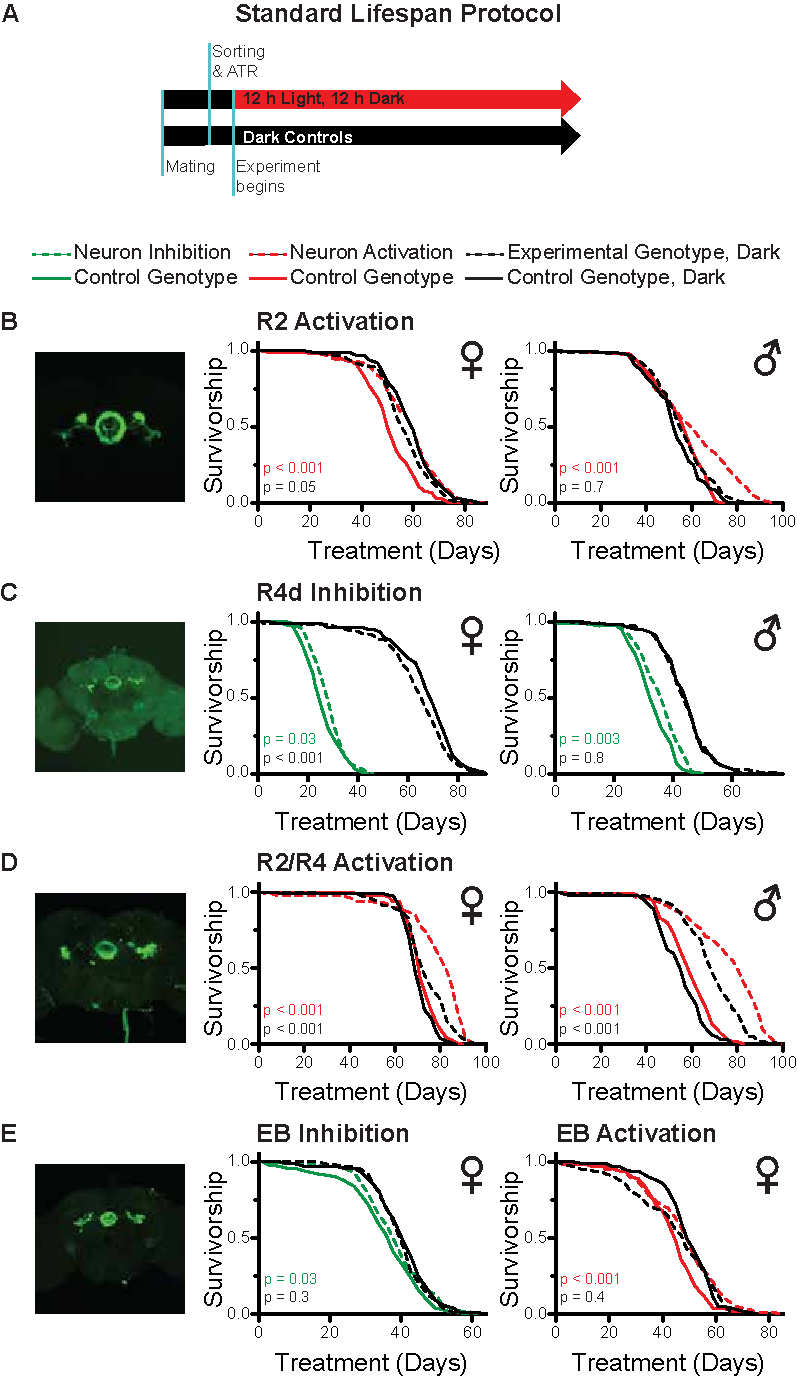
\includegraphics[width=\textwidth,height=.9\textheight,keepaspectratio]{Figs/Lifespan_Fig.pdf}
\caption{\textbf{EB manipulations extend lifespan.} Manipulation of ellipsoid body neurons R2 and R4 extends lifespan in males and females. 
(a) Flies were mated for two days, then separated by sex and sorted onto all-trans retinal food for 24 hours before optogenetic treatment began. 
(b--d) (Left) Expression patterns of drivers used in each experiment. Neurons were either activated (red lines) using UAS-CsChrimson, or inhibited (green lines) using UAS-GtACR1. Dark controls (black lines) were included for all experiments.}
\label{fig:lifespanfig}
\end{figure}

\begin{figure}[p]
\centering
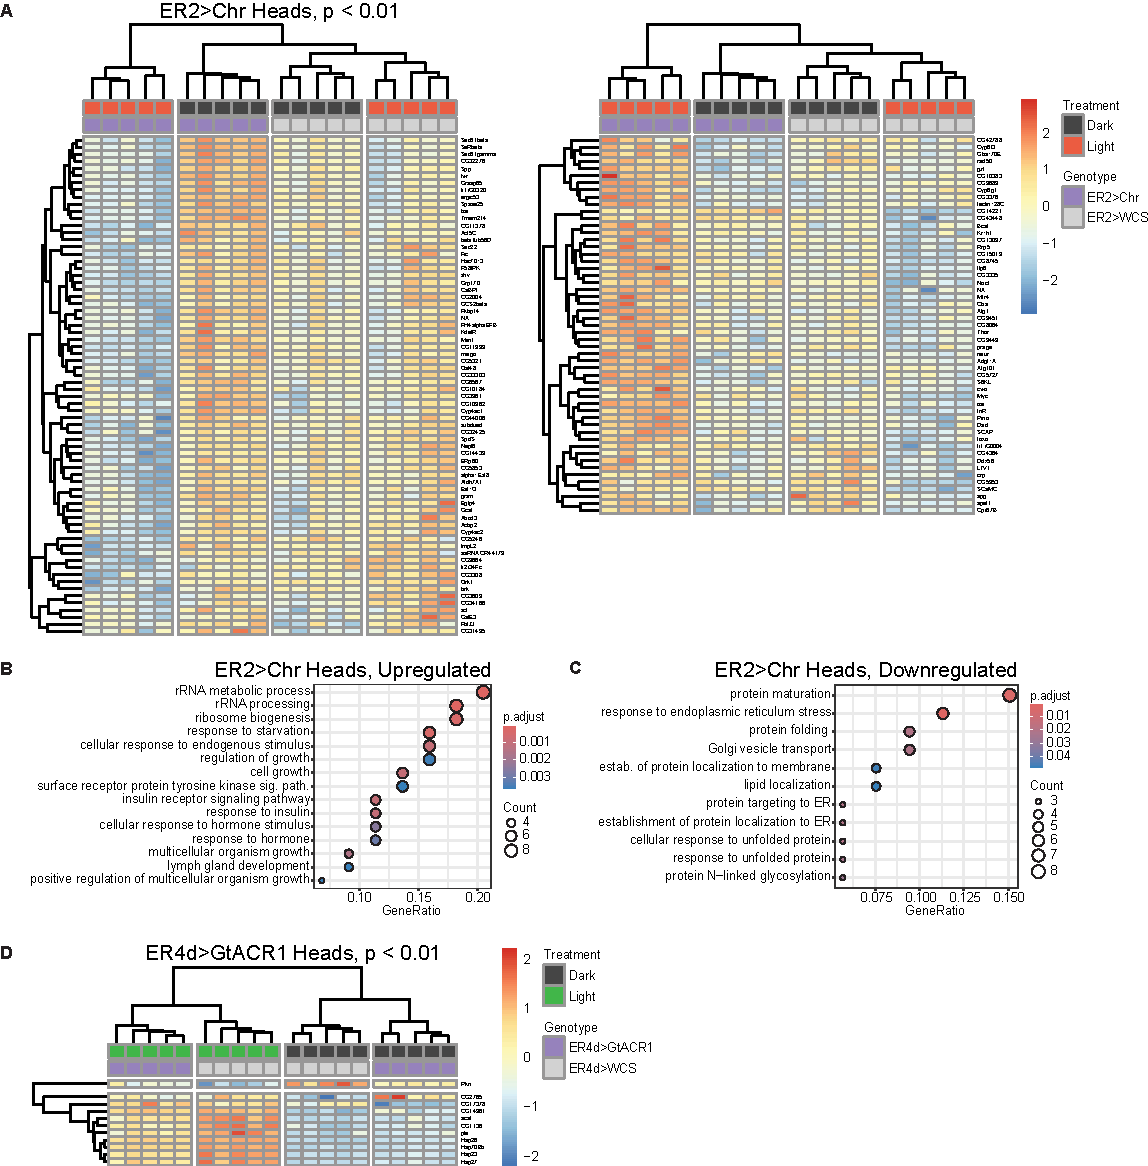
\includegraphics[width=\textwidth,height=.9\textheight,keepaspectratio]{Figs/Seq_Fig.pdf}
\caption{\textbf{EB manipulations produce distinct head transcriptomes.} Blah blah blah.}
\label{fig:seqfig}
\end{figure}

\begin{figure}[htbp]
\centering
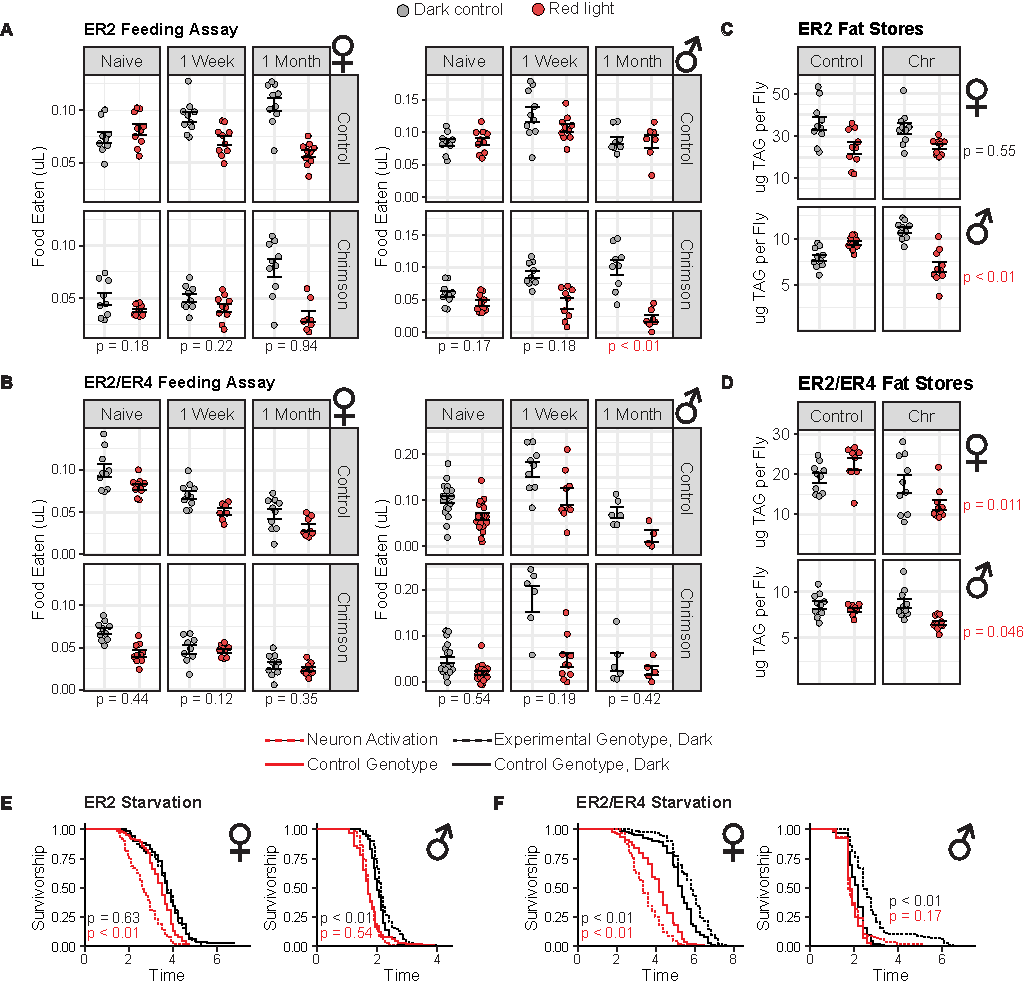
\includegraphics[width=\textwidth,height=.9\textheight,keepaspectratio]{Figs/Con-Ex_and_TAG_Fig.pdf}
\caption{\textbf{R2 and R2/R4 activation uncouples nutrient-state signaling from behavioral and physiological outputs.} \textbf{(A-D)} Interaction (Light $\times$ Genotype) p-values derived from 2-way ANOVAs. Benjamini-Hochberg correction was applied within each sex and driver, and across time points for con-ex. Female TAG points represent 5 flies; all others represent 10 flies. 
\textbf{(A)} R2-GAL4 con-ex. Female n = 8--10; male n = 7--10. 
\textbf{(B)} R2/R4-GAL4 con-ex. Female n = 7--10; male n = 18--20 (naive), 6--10 (1 week), 4--6 (1 month). 
\textbf{(C)} R2-GAL4 TAG levels. n = 10 for both sexes. 
\textbf{(D)} R2/R4-GAL4 TAG levels. Female n = 9--10; male n = 8--10. 
\textbf{(E)} R2 starvation stats. 
\textbf{(F)} R2/R4 starvation stats.}
\label{fig:conexfig}
\end{figure}

\begin{figure}[htbp]
\centering
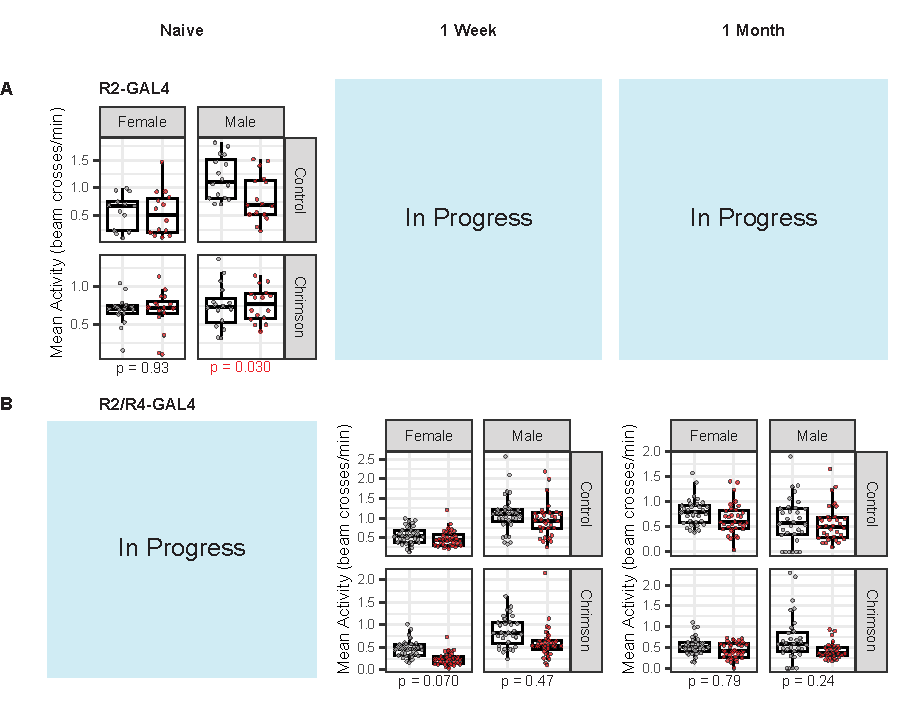
\includegraphics[scale=1]{Figs/DAMS_Fig.pdf}
\caption{\textbf{R2 and R2/R4 activaiton does not significantly affect motor activity.} R2 n = 13-16. R2/R4 n = 32. Interaction (Light $\times$ Genotype) p-values derived from 2-way ANOVAs. Benjamini-Hochberg correction was applied within each sex and driver and across time points.}
\label{fig:damsfig}
\end{figure}

\begin{figure}[htbp]
\centering
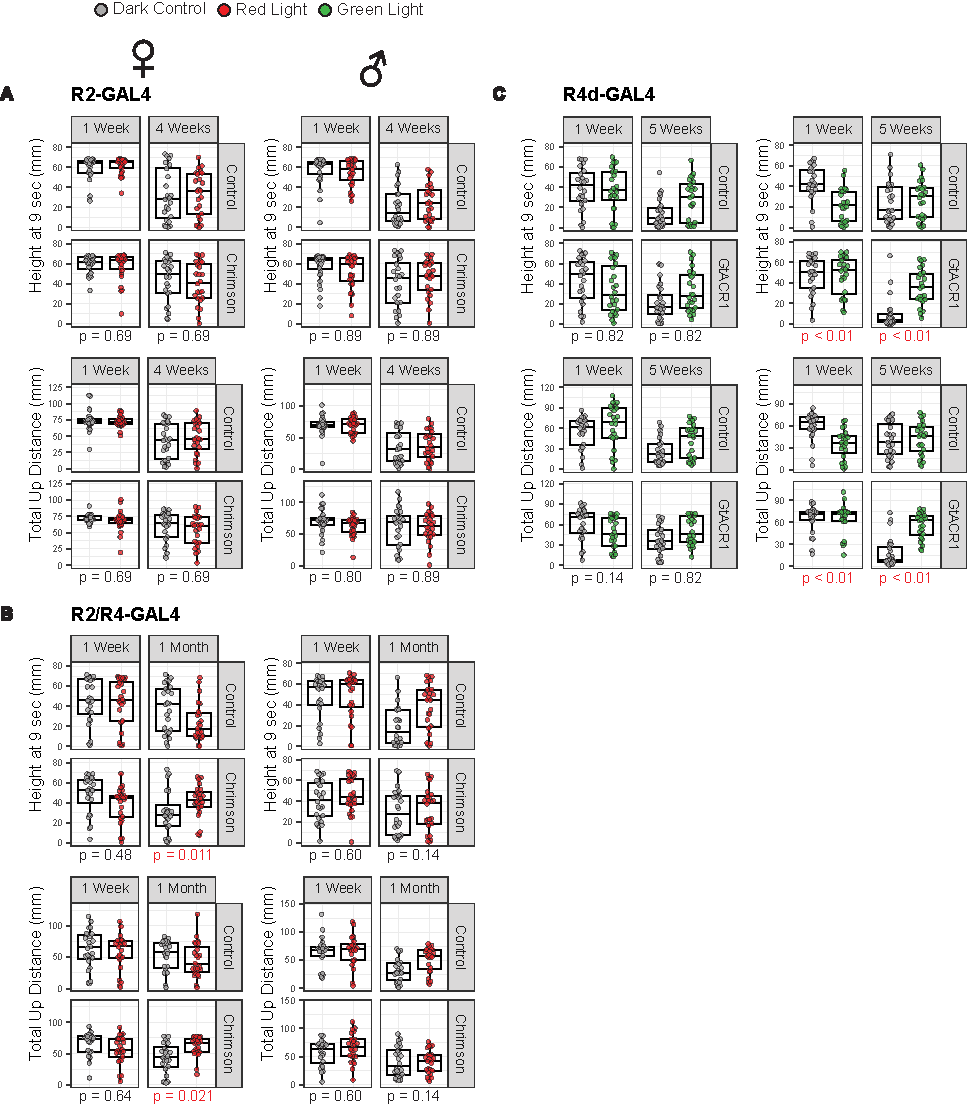
\includegraphics[scale=1]{Figs/DDrop_Fig.pdf}
\caption{\textbf{EB manipulation does not impair climbing ability.} Interaction (Light $\times$ Genotype) p-values derived from 2-way ANOVAs. Benjamini-Hochberg correction was applied within each sex and driver and across time points and climbing metrics. Points represent average of 3 trials per individual. n = 23--28.}
\label{fig:ddropfig}
\end{figure}

\begin{figure}[htbp]
\centering
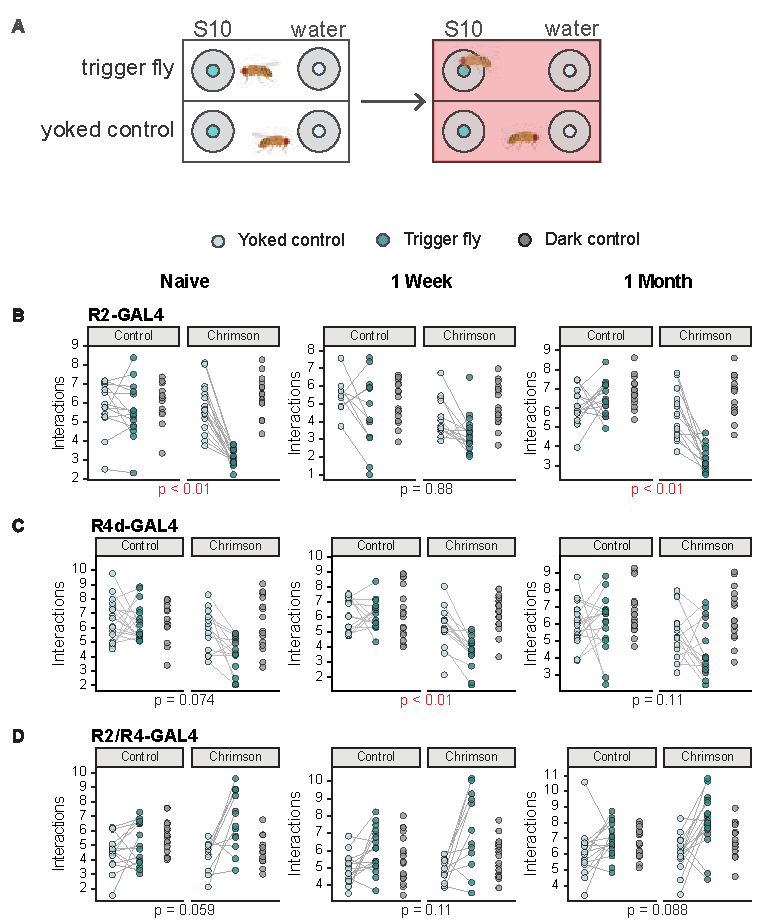
\includegraphics[scale=1]{Figs/FLIC_Fig.pdf}
\caption{\textbf{FLIC captures distinct valence states induced by EB manipulation.} Followed by desc.}
\label{fig:flicfig}
\end{figure}

\begin{figure}[p]
\centering
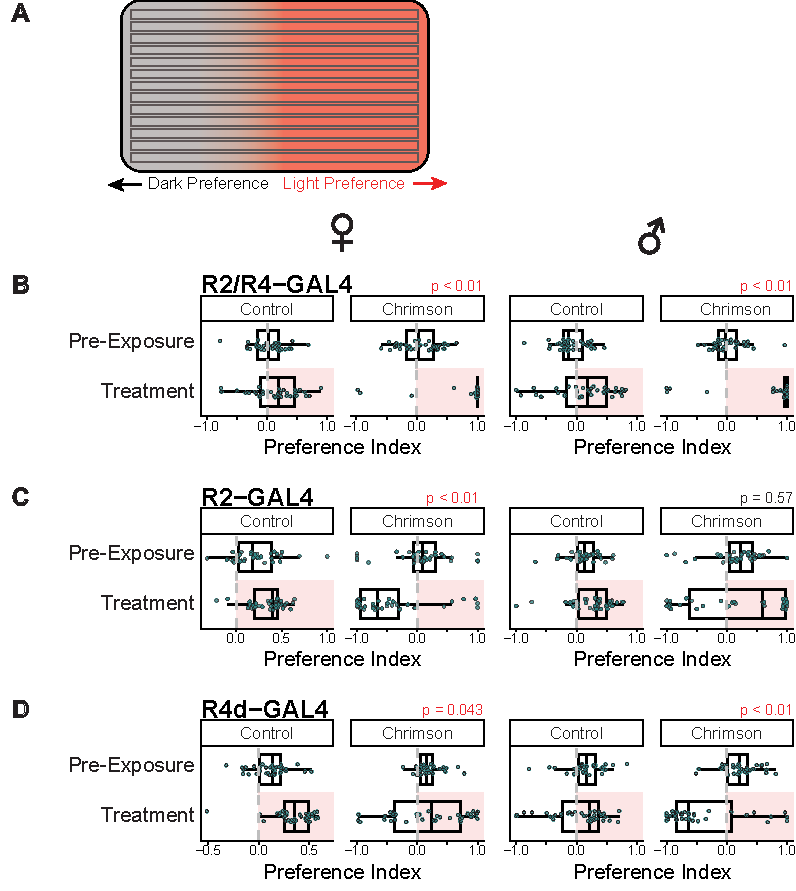
\includegraphics[width=\textwidth,height=.9\textheight,keepaspectratio]{Figs/Arena_Fig.pdf}
\caption{\textbf{Valence of EB manipulation is sex-, circuit-, and context-dependent.} Blah blah arena.}
\label{fig:arenafig}
\end{figure}
% =========================
% Supplement
% =========================

\clearpage
\onecolumn  % remove if you want supplement to stay two-column

\setcounter{figure}{0}
\renewcommand{\thefigure}{S\arabic{figure}}

\setcounter{table}{0}
\renewcommand{\thetable}{S\arabic{table}}

\setcounter{equation}{0}
\renewcommand{\theequation}{S\arabic{equation}}

\section*{Supplemental Figures}

\begin{figure*}[htbp]
  \centering
  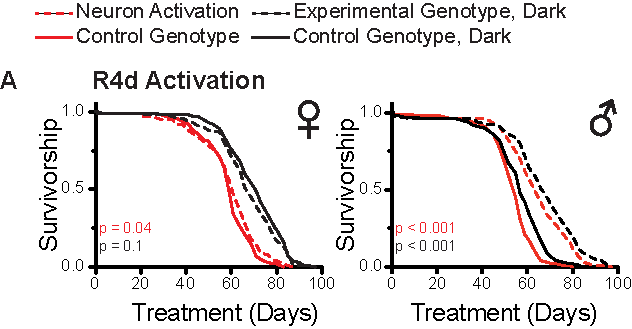
\includegraphics[scale=1]{Figs/Lifespan_Supp.pdf}
  \caption{\textbf{Lifespan supplement.} Followed by desc.}
  \label{fig:lifespansupp}
\end{figure*}

\begin{figure*}[htbp]
  \centering
  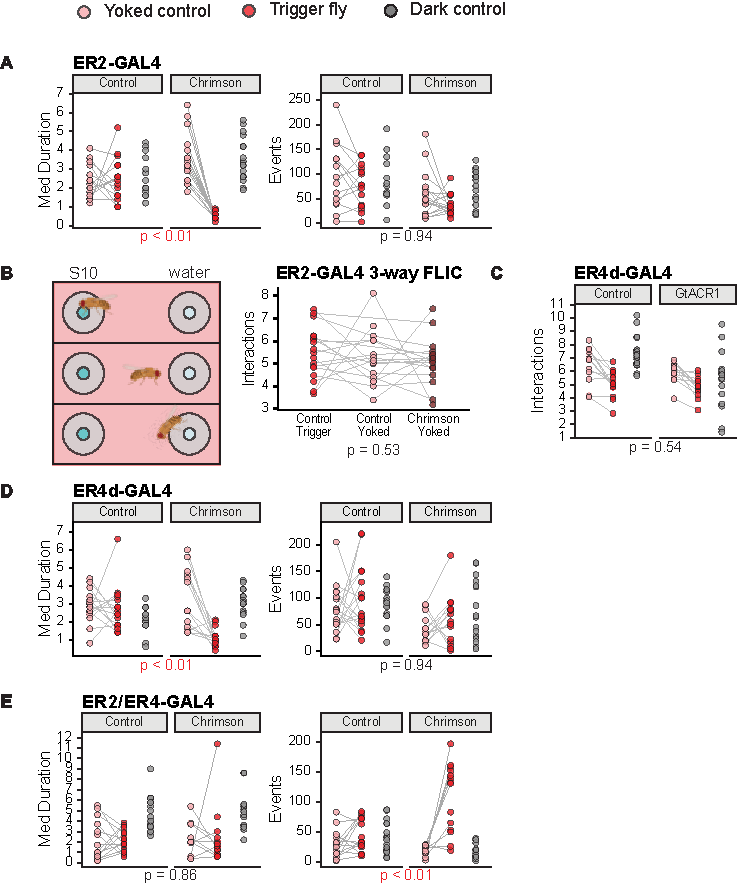
\includegraphics[scale=1]{Figs/FLIC_Supp.pdf}
  \caption{\textbf{FLIC supplement.} Followed by desc.}
  \label{fig:flicsupp}
\end{figure*}

\begin{figure*}[htbp]
  \centering
  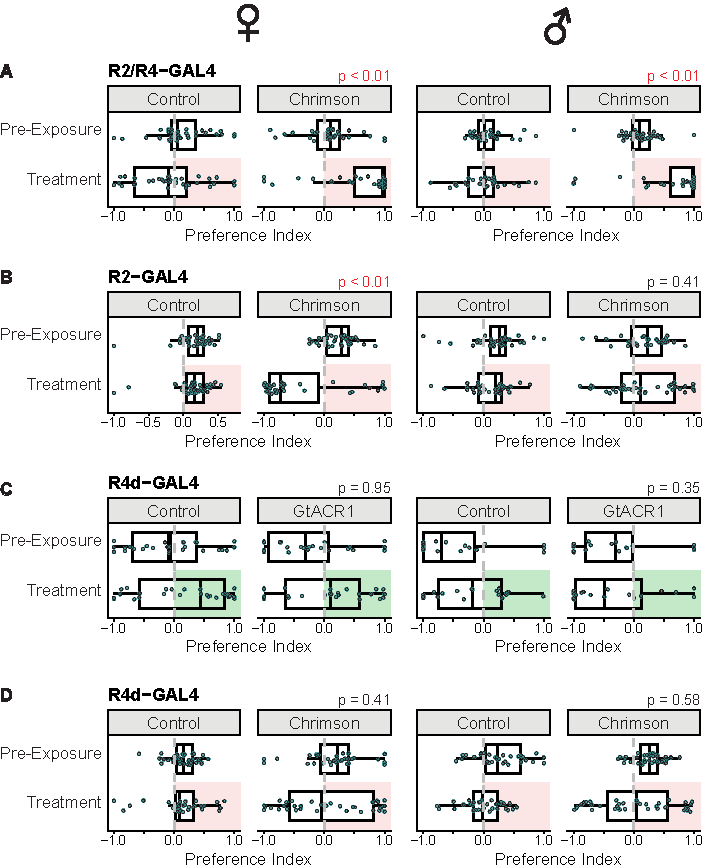
\includegraphics[scale=1]{Figs/Arena_Supp.pdf}
  \caption{\textbf{Arena supplement.} Followed by desc.}
  \label{fig:arenasupp}
\end{figure*}
R4d>Chr (Supp):
-	Only diff is 1 week ixn, males and females, for total up distance; exp females worse, ctrl males worse
\begin{figure*}[htbp]
  \centering
  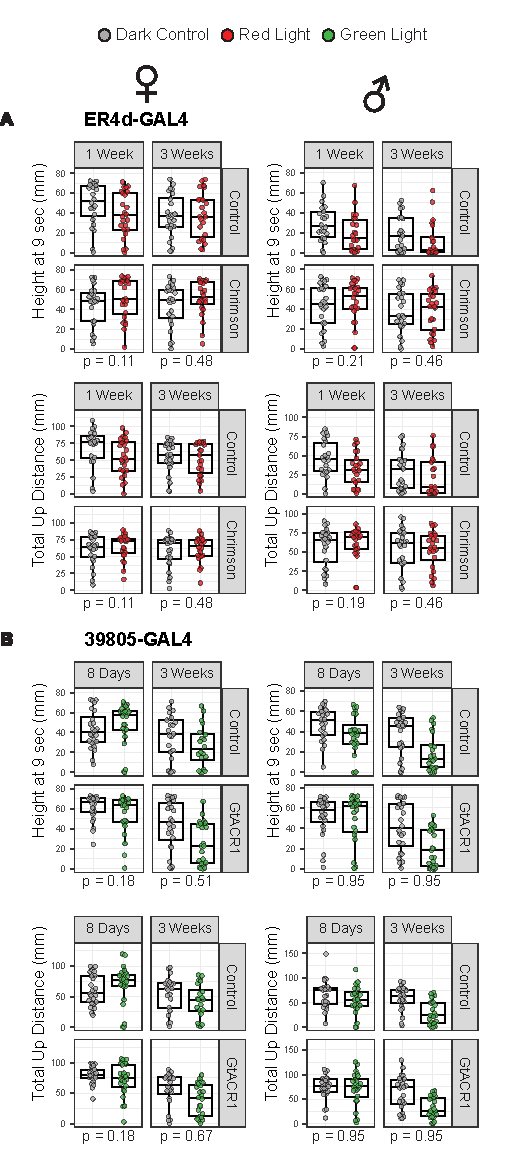
\includegraphics[scale=1]{Figs/DDrop_Supp.pdf}
  \caption{\textbf{DDrop supplement.} n = 20-24.}
  \label{fig:ddropsupp}
\end{figure*}

\end{document}